%%%%%%%%%%%%%%%%%%%%%%%%%%%%%%%%%%%%%%%%%
% Beamer Presentation
% LaTeX Template
% Version 1.0 (10/11/12)
%
% This template has been downloaded from:
% http://www.LaTeXTemplates.com
%
% License:
% CC BY-NC-SA 3.0 (http://creativecommons.org/licenses/by-nc-sa/3.0/)
%
%%%%%%%%%%%%%%%%%%%%%%%%%%%%%%%%%%%%%%%%%

%----------------------------------------------------------------------------------------
%	PACKAGES AND THEMES
%----------------------------------------------------------------------------------------

\documentclass[14pt]{beamer}
\usefonttheme[onlymath]{serif}

\mode<presentation> {

% The Beamer class comes with a number of default slide themes
% which change the colors and layouts of slides. Below this is a list
% of all the themes, uncomment each in turn to see what they look like.

\usetheme{default}
%\usetheme{AnnArbor}
%\usetheme{Antibes}
%\usetheme{Bergen}
%\usetheme{Berkeley}
%\usetheme{Berlin}
%\usetheme{Boadilla}
%\usetheme{CambridgeUS}
%\usetheme{Copenhagen}
%\usetheme{Darmstadt}
%\usetheme{Dresden}
%\usetheme{Frankfurt}
%\usetheme{Goettingen}
%\usetheme{Hannover}
%\usetheme{Ilmenau}
%\usetheme{JuanLesPins}
%\usetheme{Luebeck}
%\usetheme{Madrid}
%\usetheme{Malmoe}
%\usetheme{Marburg}
%\usetheme{Montpellier}
%\usetheme{PaloAlto}
%\usetheme{Pittsburgh}
%\usetheme{Rochester}
%\usetheme{Singapore}
%\usetheme{Szeged}
%\usetheme{Warsaw}

% As well as themes, the Beamer class has a number of color themes
% for any slide theme. Uncomment each of these in turn to see how it
% changes the colors of your current slide theme.

%\usecolortheme{albatross}
%\usecolortheme{beaver}
%\usecolortheme{beetle}
%\usecolortheme{crane}
%\usecolortheme{dolphin}
%\usecolortheme{dove}
%\usecolortheme{fly}
%\usecolortheme{lily}
%\usecolortheme{orchid}
%\usecolortheme{rose}
%\usecolortheme{seagull}
%\usecolortheme{seahorse}
%\usecolortheme{whale}
%\usecolortheme{wolverine}

%\setbeamertemplate{footline} % To remove the footer line in all slides uncomment this line
%\setbeamertemplate{footline}[page number] % To replace the footer line in all slides with a simple slide count uncomment this line

%\setbeamertemplate{navigation symbols}{} % To remove the navigation symbols from the bottom of all slides uncomment this line
}

\usepackage{color} % colored text
%\usepackage{graphicx} % Allows including images
%\usepackage{grffile}
%\usepackage{booktabs} % Allows the use of \toprule, \midrule and \bottomrule in tables
%\usepackage{caption}
\usepackage{subcaption}
\captionsetup{compatibility=false}
%\usepackage{lmodern}
\usepackage{siunitx}
\sisetup{separate-uncertainty=true}
\sisetup{multi-part-units=single}
\usepackage{tikz}
\usepackage{feynmp-auto}
\usepackage{hepnames}
\usepackage{mhchem}

\graphicspath{{figures/}}

%----------------------------------------------------------------------------------------
%	TITLE PAGE
%----------------------------------------------------------------------------------------

% The short title appears at the bottom of every slide, the full title is only
% on the title page
\title[KamLAND]{High Energy Analysis at KamLAND\\ and\\ Application to Dark
	Matter Search}

\author{Michinari Sakai} % Your name
\institute[UH] % Your institution as it will appear on the bottom of every slide, may be shorthand to save space
{
University of Hawaii, Manoa \\ % Your institution for the title page
\medskip
\textit{michinar@hawaii.edu} % Your email address
}
\date{\today} % Date, can be changed to a custom date

\begin{document}

\begin{frame}
\titlepage % Print the title page as the first slide
\end{frame}

\begin{frame}
\frametitle{Overview} % Table of contents slide, comment this block out to remove it
\tableofcontents % Throughout your presentation, if you choose to use \section{} and \subsection{} commands, these will automatically be printed on this slide as an overview of your presentation
\end{frame}

%----------------------------------------------------------------------------------------
%	PRESENTATION SLIDES
%----------------------------------------------------------------------------------------

%------------------------------------------------
%\section{First Section} % Sections can be created in order to organize your presentation into discrete blocks, all sections and subsections are automatically printed in the table of contents as an overview of the talk
%------------------------------------------------

%\subsection{Subsection Example} % A subsection can be created just before a set of slides with a common theme to further break down your presentation into chunks

\begin{frame}[t]{KamLAND: $\nu$ detector in Japan}
	\centering
	\begin{figure}
		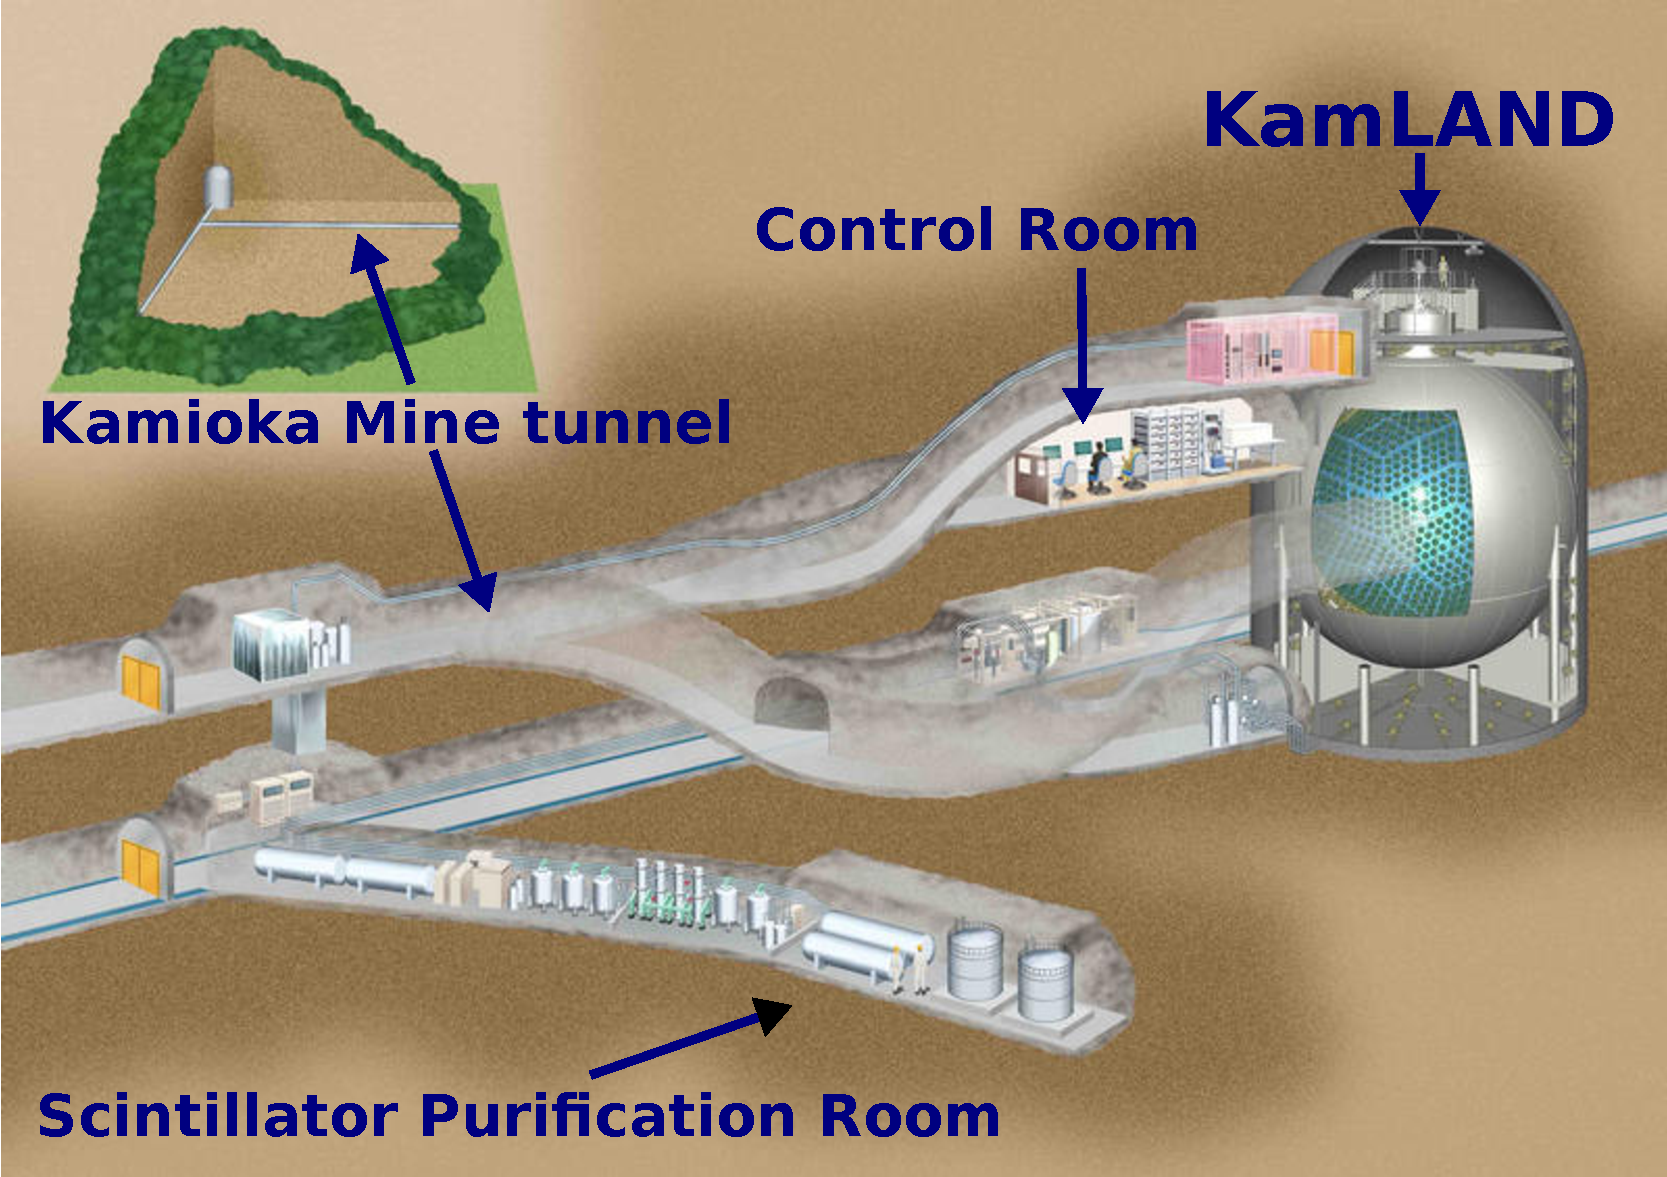
\includegraphics[width=\linewidth]{kamland_tunnel.pdf}
	\end{figure}
\end{frame}

\section{Introduction}
\begin{frame}[t]{KamLAND: features}
	\begin{itemize}
		\item<1-> Commissioned: \num{2001}
		\item<1-> Detector medium: liquid scintillator
		\item<1-> Size: \SI{1}{\kilo\tonne}
		\item<1-> Photomultiplier tubes:\\
			\num{1325} 17-inch, \num{779} 20-inch
			(Hamamatsu), \SI{34}{\percent} photo-coverage
		\item<1-> Analysis $\nu$ energy: $\sim\si{\mega\electronvolt}$
		\item<1-> Energy resolution: \SI{7.0\pm0.1}{\percent}
		\item<1-> Vertex resolution:
			\SI{13.8\pm2.3}{\centi\meter\per\sqrt{E(\mega\electronvolt)}}
		\item<2-> {\color{red}Directional sensitivity: NONE}
		\item<3-> {\color{red}No analysis at higher energies}
	\end{itemize}
\end{frame}

\section{Neutrino directionality}
\subsection{Issues}
\begin{frame}{Directionality in water}
	\centering
	\begin{columns}[T]
		\column{0.5\linewidth}
		\begin{block}{\centering{Super-Kamiokande}}
			\begin{tikzpicture}
				\node (img1)
				{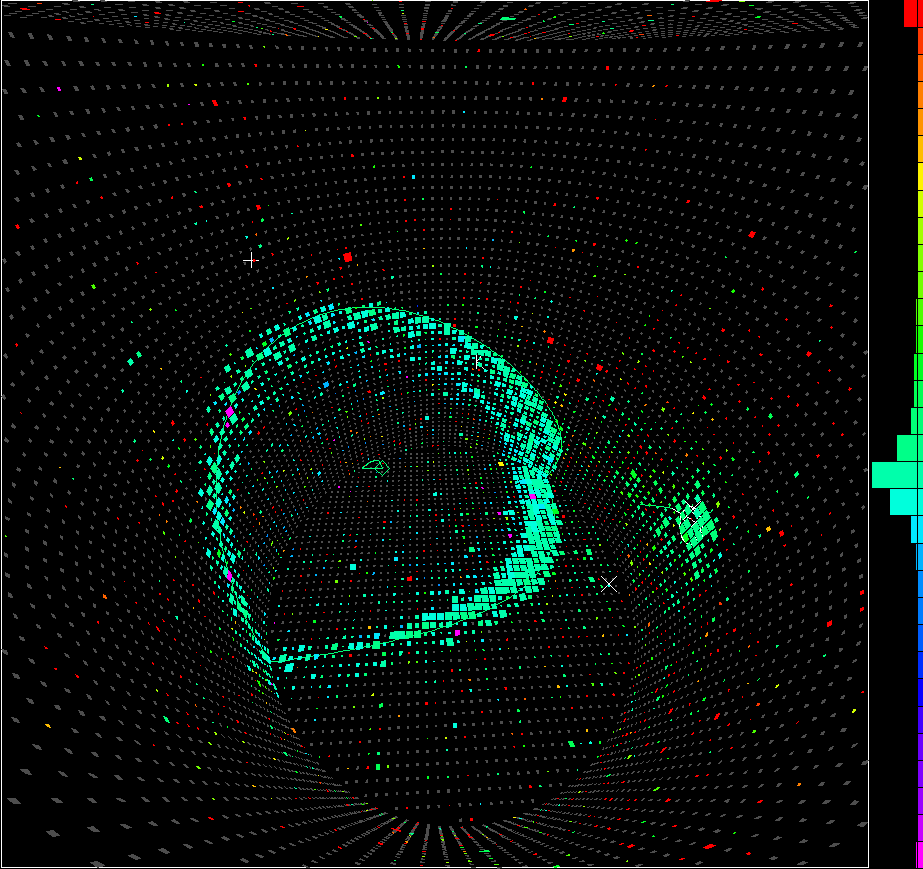
\includegraphics[width=\linewidth]{sk_cherenkov_ring.png}};
				\pause
				\node (img2) at (img1)
				{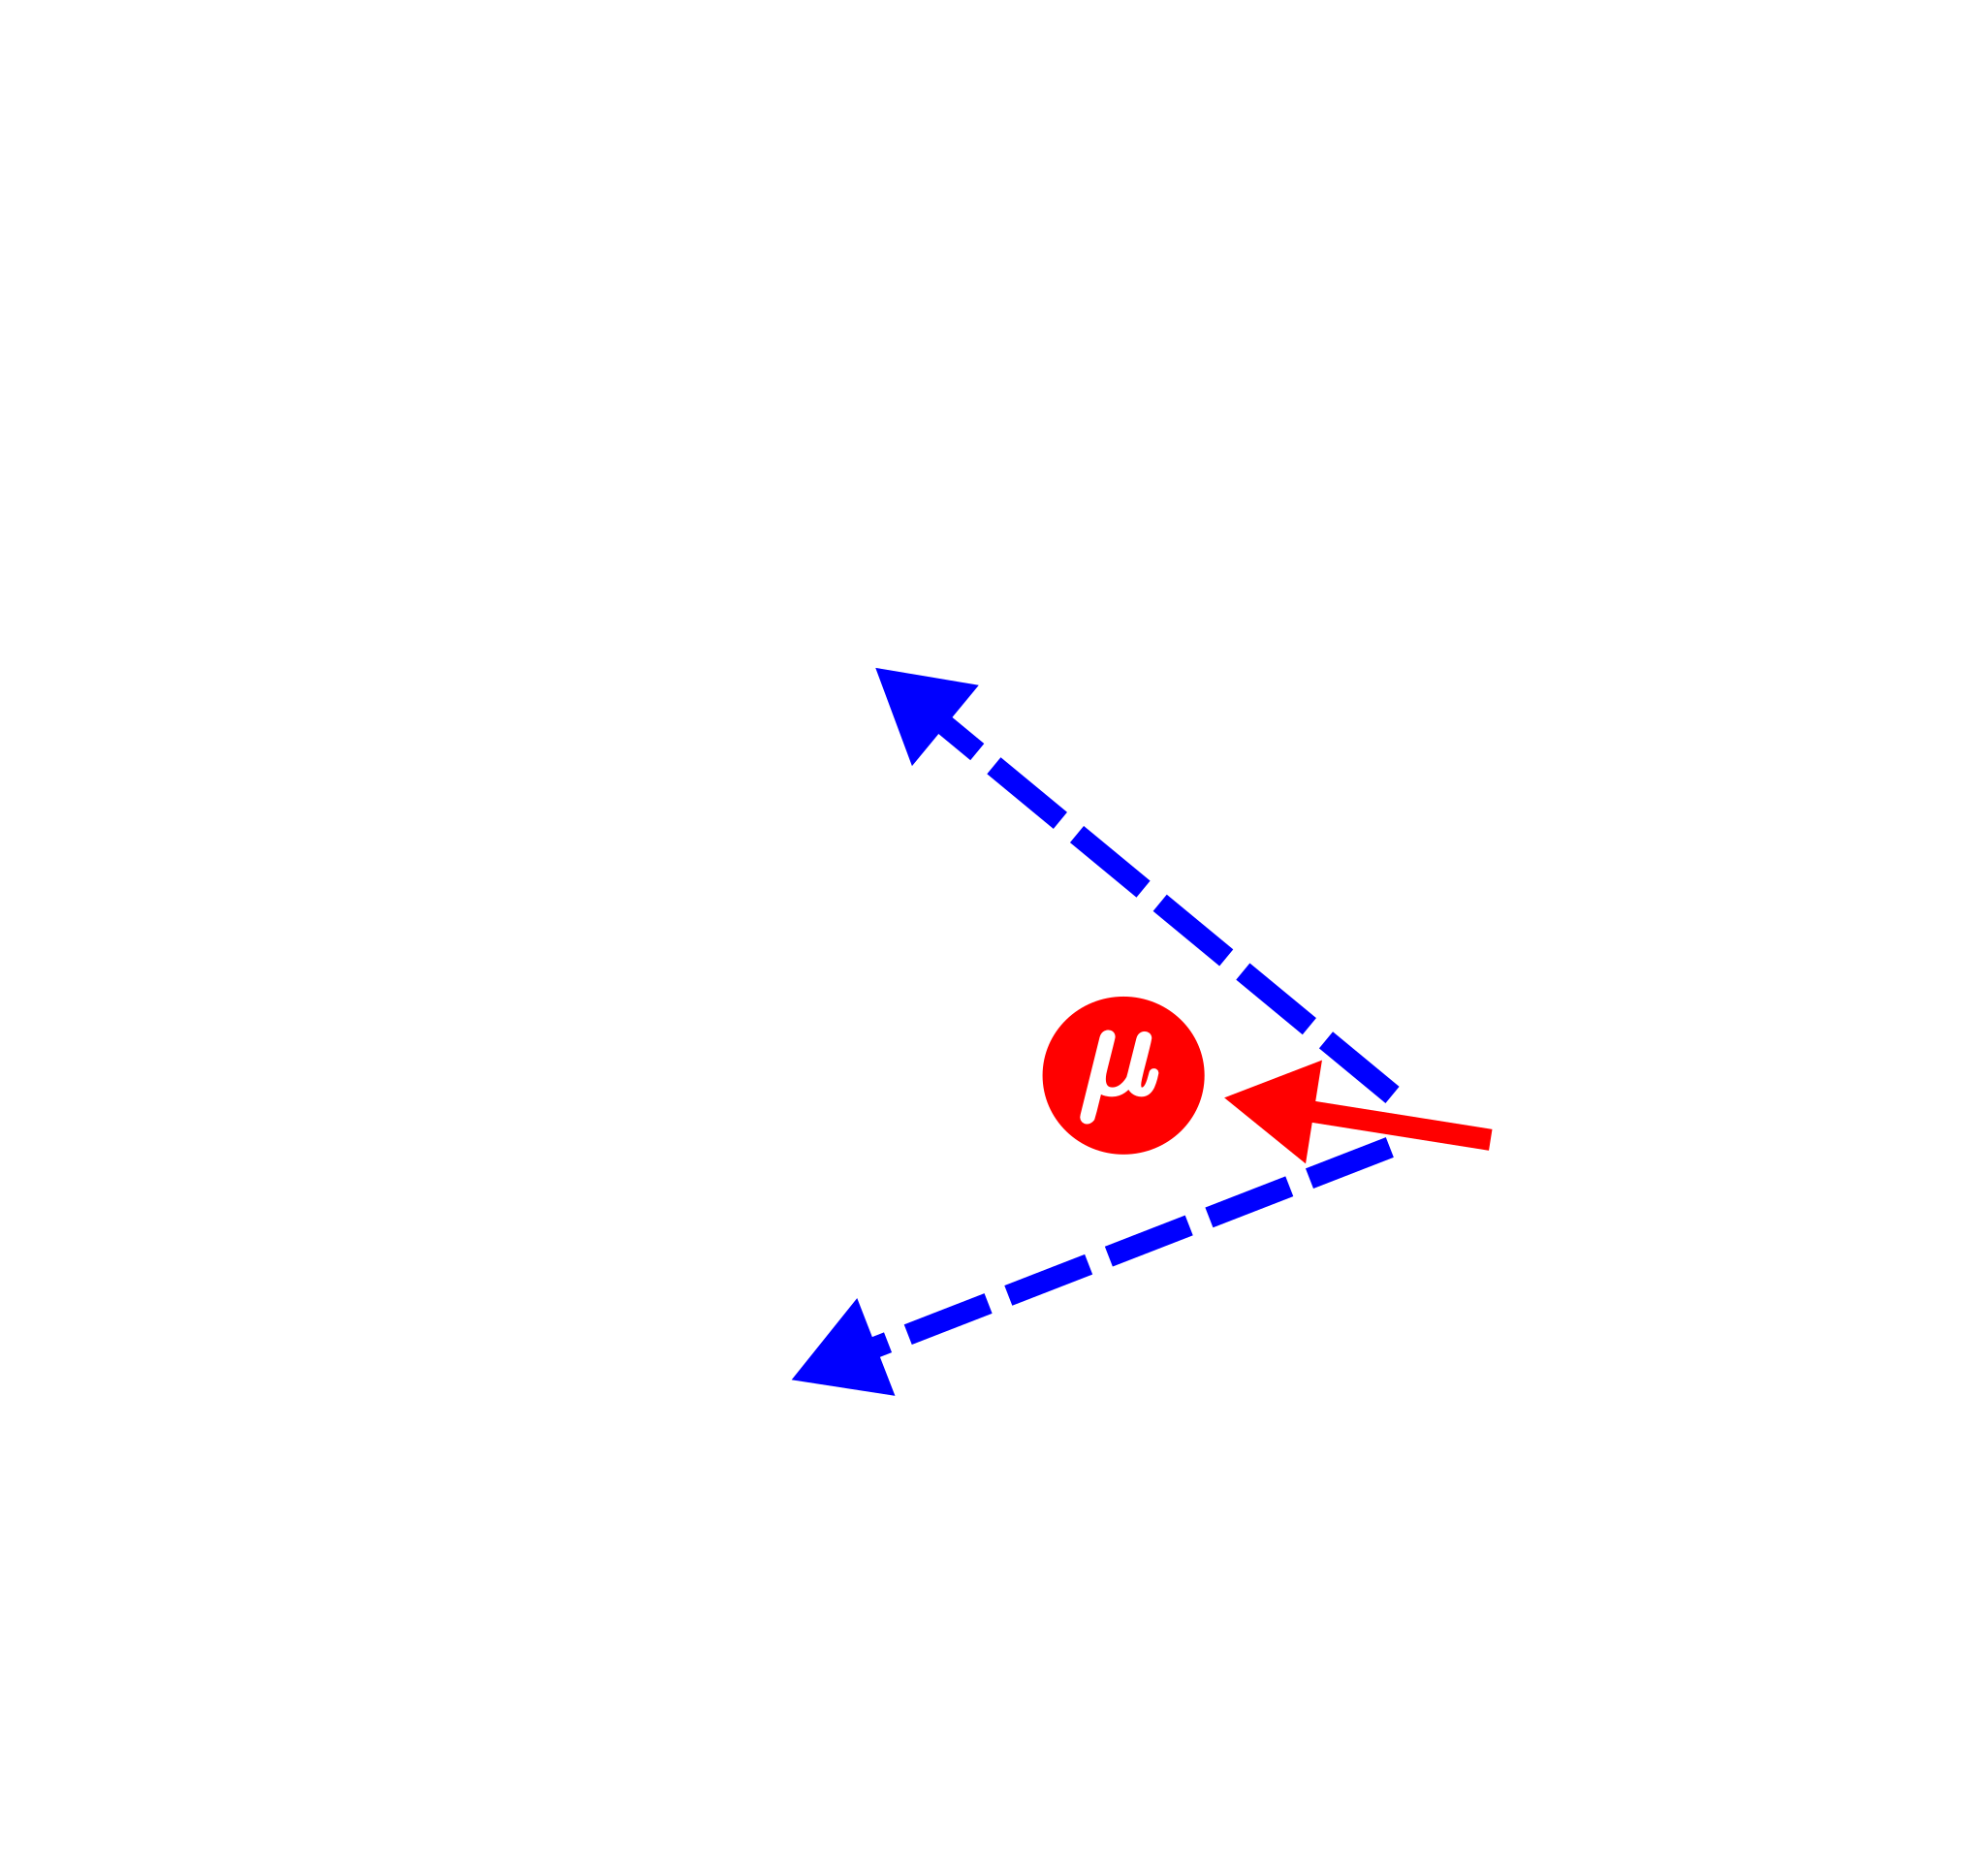
\includegraphics[width=\linewidth]{sk_cherenkov_ring_with_lepton.png}};
			\end{tikzpicture}
		\end{block}
		\column{0.5\linewidth}
		\begin{block}{}
			\begin{itemize}
				\item<1-> Cherenkov rings
				\item<2-> Tell charged particle direction
				\item<3-> {\color{blue}Can we do something similar in
					scintillator?}
			\end{itemize}
		\end{block}
	\end{columns}
\end{frame}

\begin{frame}{In scintillator...}
	\centering
	\begin{columns}[T]
		\column{0.5\linewidth}
		\begin{block}{\centering{KamLAND}}
			\begin{tikzpicture}
				\node (img1)
				{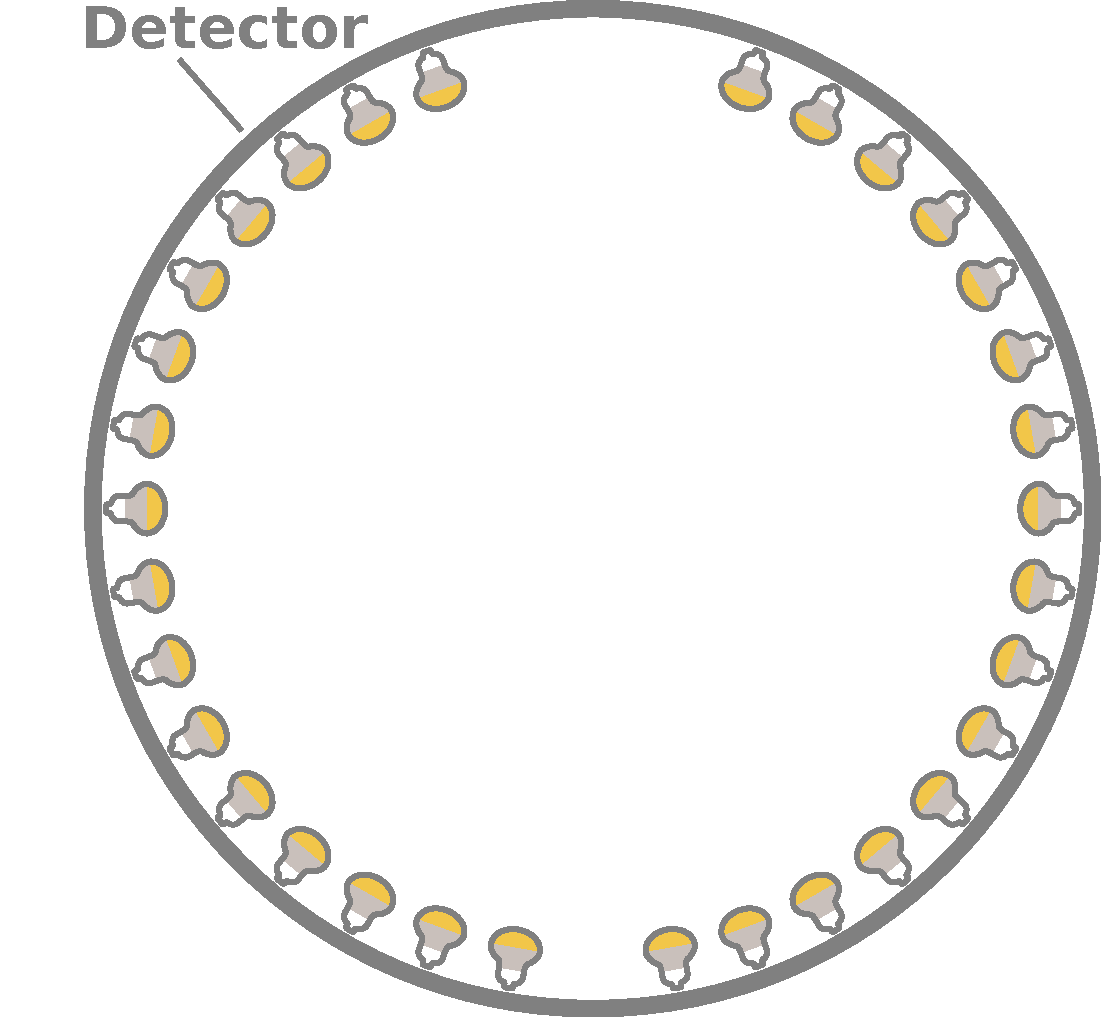
\includegraphics[width=\linewidth]{kl_fermat_surface_with_lepton-detector.pdf}};
				\pause
				\node (img2) at (img1)
				{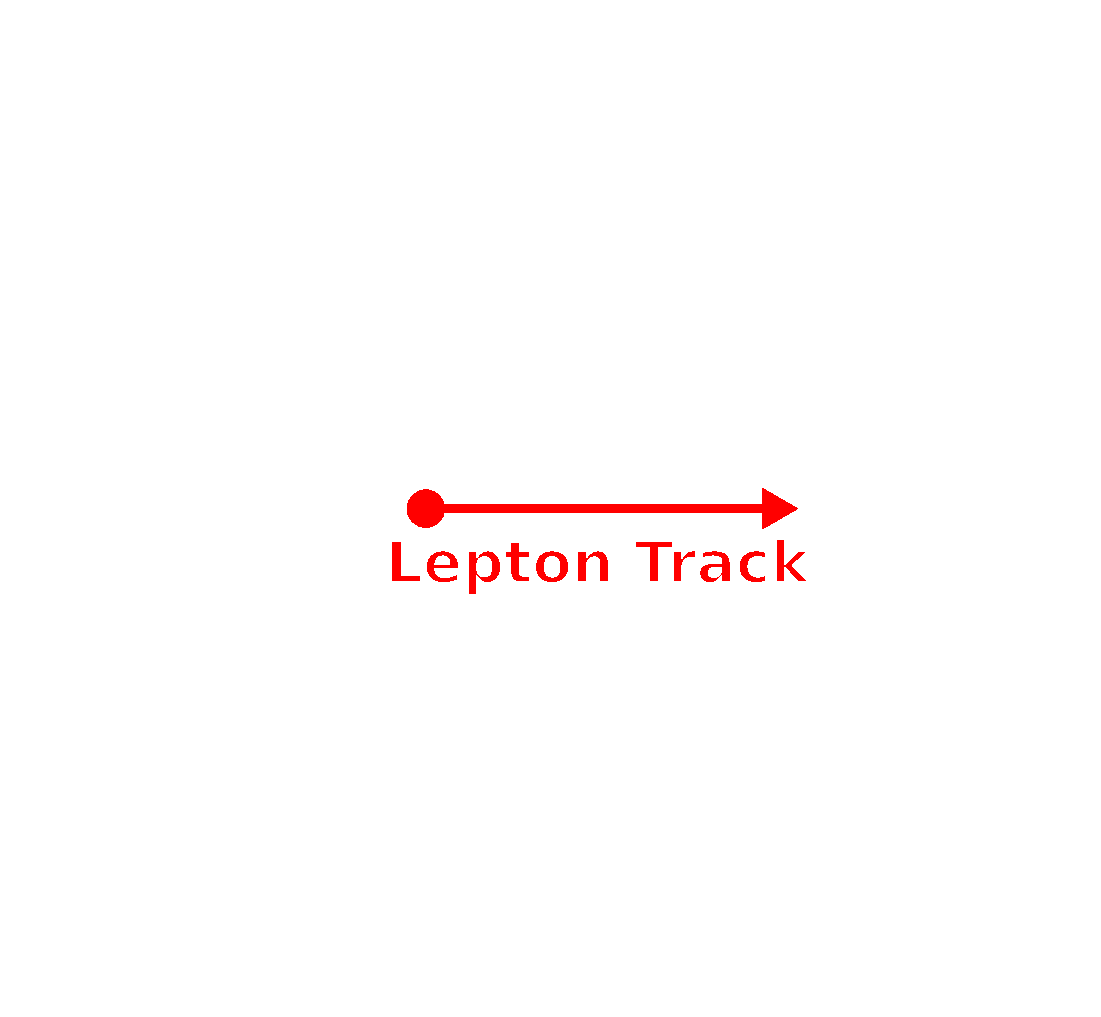
\includegraphics[width=\linewidth]{kl_fermat_surface_with_lepton-lepton_track.pdf}};
				\pause
				\node (img3) at (img1)
				{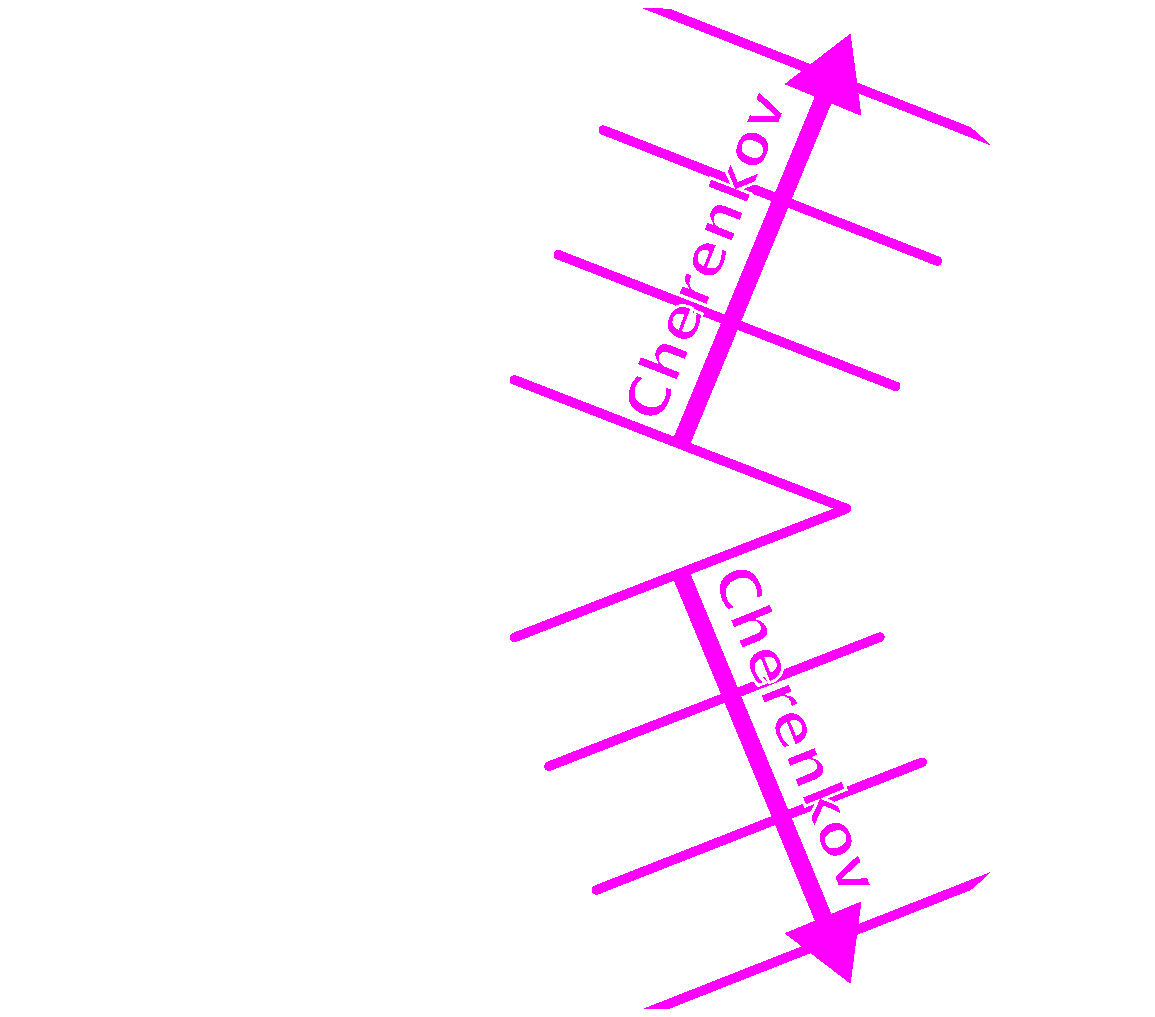
\includegraphics[width=\linewidth]{kl_fermat_surface_with_lepton-cherenkov.pdf}};
				\pause
				\node (img4) at (img1)
				{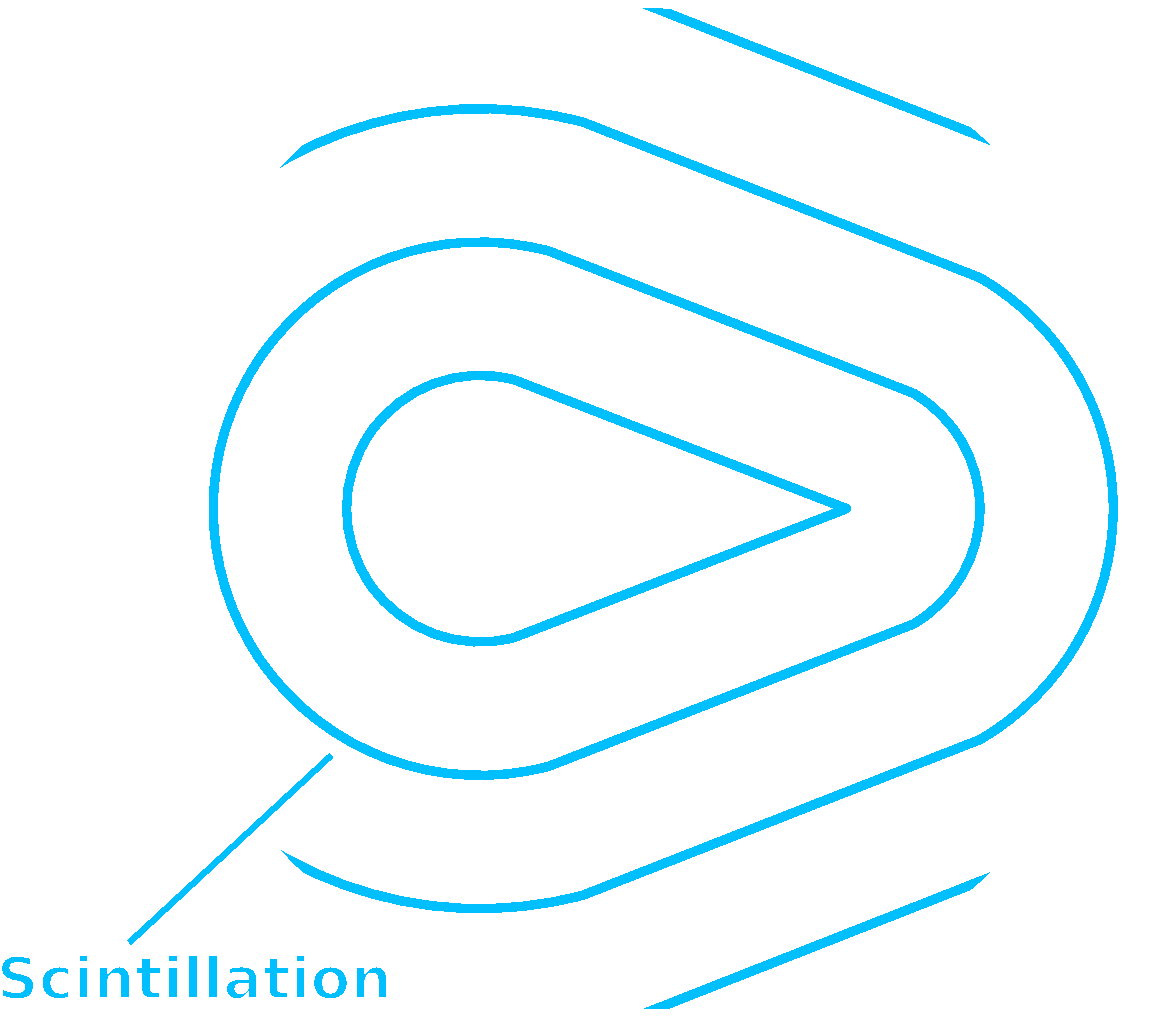
\includegraphics[width=\linewidth]{kl_fermat_surface_with_lepton-scintillation.pdf}};
			\end{tikzpicture}
		\end{block}
		\column{0.5\linewidth}
		\begin{block}{}
			\begin{itemize}
				\item<3-> Cherenkov is emitted
				\item<4-> Along with isotropic Scintillation
				\item<5-> {\color{red}$\implies$ Cannot simply use Cherenkov
					for directionality}
			\end{itemize}
		\end{block}
	\end{columns}
\end{frame}

\begin{frame}[fragile]{Furthermore...}
	\centering
	\begin{columns}[T]
		\column{0.5\linewidth}
		\begin{block}{\centering{Inverse-beta decay}\\~\\}
			\centering
			\begin{fmffile}{inverse_beta_decay} \begin{fmfgraph*}(150,120)
				\fmfpen{thick}
				\fmfleft{i1,i2} \fmfright{o1,o2}
				\fmf{fermion,label=\Pproton}{i1,v1}
				\fmf{fermion,label=\Pneutron}{v1,o1}
				\fmf{fermion,label=\APnue}{i2,v2}
				\fmf{fermion,label=\Ppositron}{v2,o2}
				\fmf{boson,label=\PWminus}{v1,v2}
				\fmfblob{1cm}{v1}
			\end{fmfgraph*} \end{fmffile}
		\end{block}
		\column{0.5\linewidth}
		\begin{block}{}
			\begin{itemize}
				\item<2-> KamLAND is used to seeing simple kinematics at low
					energies (\si{\mega\electronvolt})
				\item<3-> single final-state lepton
			\end{itemize}
		\end{block}
	\end{columns}
\end{frame}

\begin{frame}[fragile]{But at higher energies, the kinematics is not so simple}
	\centering
	\begin{columns}[t]
		\column{0.5\linewidth}
		\begin{block}{\centering{Resonance production}\\~\\}
			\centering
			\begin{fmffile}{resonance_production} \begin{fmfgraph*}(120,120)
				\fmfpen{thick}
				\fmfleft{i1,i2} \fmfright{o1,o2,o3}
				\fmf{fermion}{i1,v1}
				\fmflabel{\Pproton}{i1}
				\fmf{fermion,label=\HepParticle{\Delta}{}{++}}{v1,v3}
				\fmf{fermion}{v3,o1}
				\fmflabel{\Pproton}{o1}
				\fmf{fermion}{v3,o2}
				\fmflabel{\Ppiplus}{o2}
				\fmf{fermion}{i2,v2,o3}
				\fmflabel{\Pnum}{i2}
				\fmflabel{\Pmuon}{o3}
				\fmf{boson,label=\PWplus}{v1,v2}
				\fmfblob{1cm}{v1}
			\end{fmfgraph*} \end{fmffile}
		\end{block}
		\column{0.5\linewidth}
		\begin{block}{\centering{\fontsize{14pt}{14pt}\selectfont{Deep inelastic
			scattering}}\\~\\}
			\begin{fmffile}{deep_inelastic_scattering} \begin{fmfgraph*}(120,120) \fmfpen{thick}
				\fmfleft{i1,i2} \fmfright{o1,o2,o3}
                \fmflabel{\Pproton}{i1}
                \fmf{plain}{i1,v1}
                \fmf{plain,label=\Pup}{v1,v3}
                \fmf{phantom}{v1,o1}
                \fmflabel{$X$}{o1}
                \fmf{plain}{v3,o2}
				\fmflabel{\Pup}{o2}
                \fmf{fermion}{i2,v2,o3}
				\fmflabel{\Pnum}{i2}
                \fmflabel{\Pmuon}{o3}
                \fmf{boson,label=\PWplus}{v2,v3}
                \fmffreeze
                \fmfi{plain}{vpath (__i1,__v1) shifted (thick*(-0.5,+2))}
                \fmfi{plain}{vpath (__i1,__v1) shifted (thick*(+0.5,-2))}
                \fmffreeze
                \fmfi{plain}{vpath (__v1,__o1) shifted (thick*(+0.25,+1))}
                \fmfi{plain}{vpath (__v1,__o1) shifted (thick*(-0.25,-1))}
                \fmfblob{1cm}{v1}
			\end{fmfgraph*} \end{fmffile}
		\end{block}
	\end{columns}
\end{frame}

\begin{frame}{Many photons at high energy in scintillator}
	\begin{columns}[T]
		\column{0.5\linewidth}
		\begin{block}{\centering{Cosmic ray $\mu$}}
			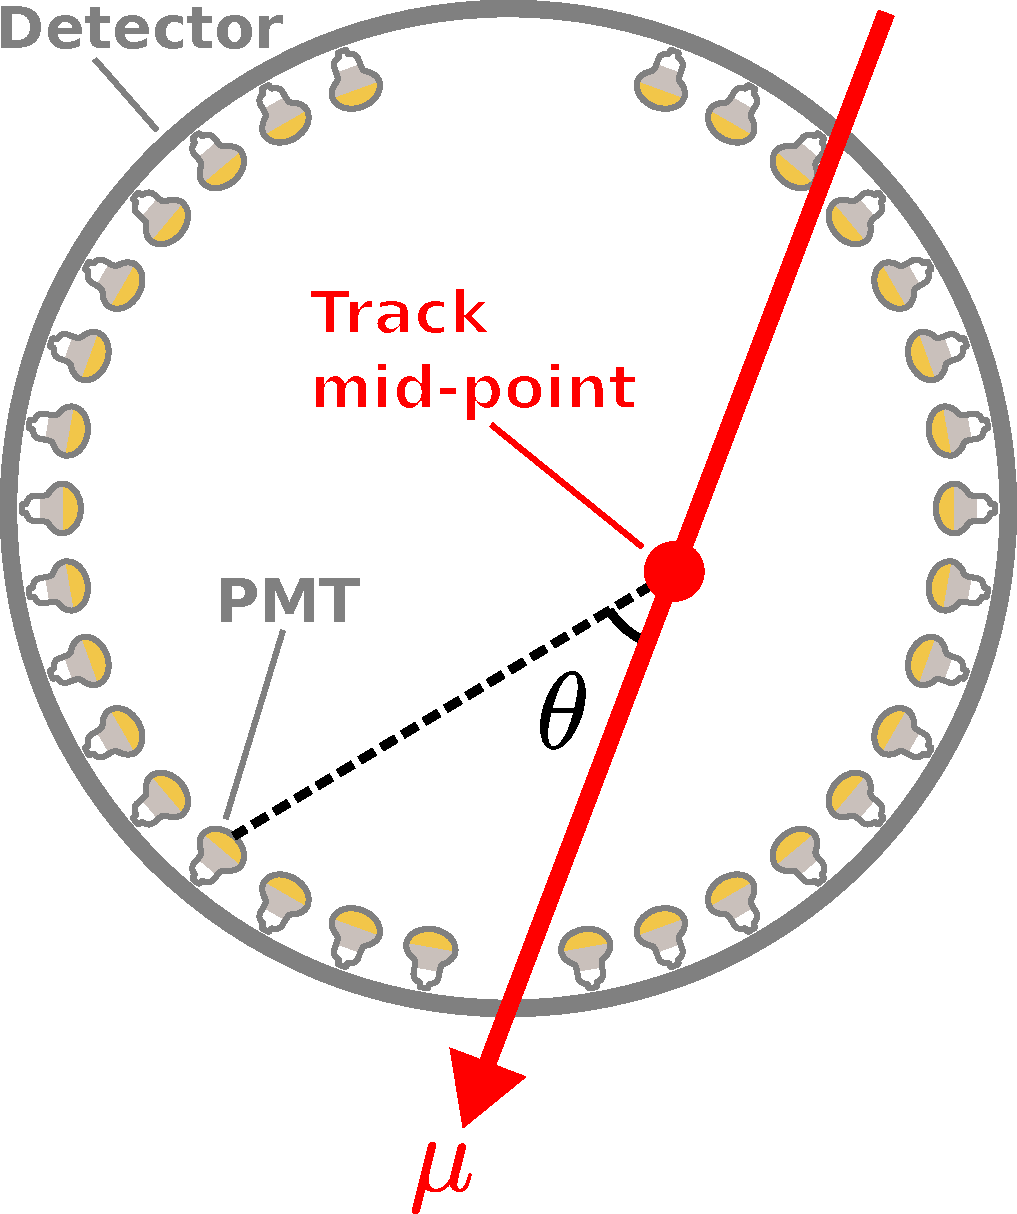
\includegraphics[width=\linewidth]{through_going_muon.pdf}
		\end{block}
		\column{0.5\linewidth}
		\begin{block}{\centering{204 $\mu$'s overlaid}}
			\begin{tikzpicture}
				\node (img1)
				{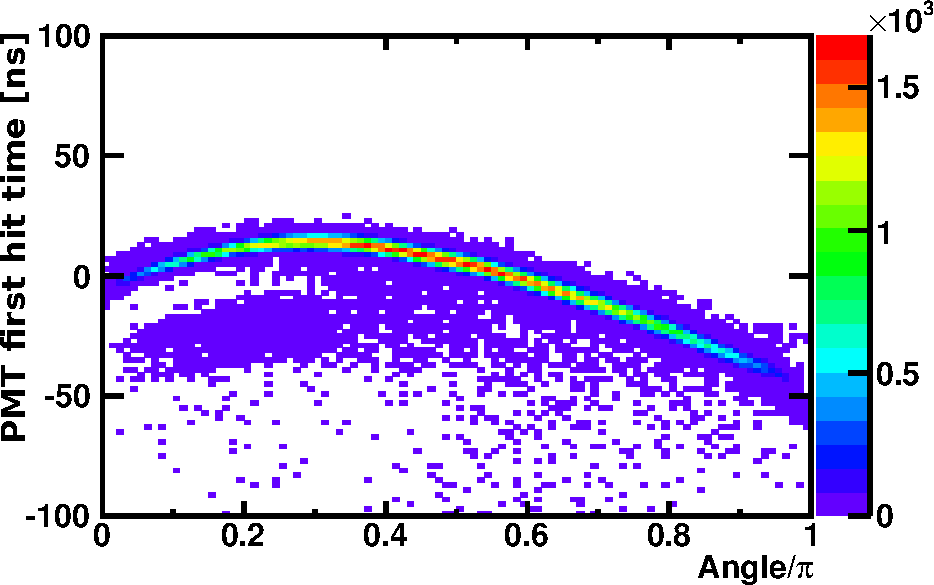
\includegraphics[width=\linewidth]{analyzed_rtq_atm_muon_run005000_test_hitTimePositions_all.pdf}};
				\pause
				\node (img2) at (img1)
				{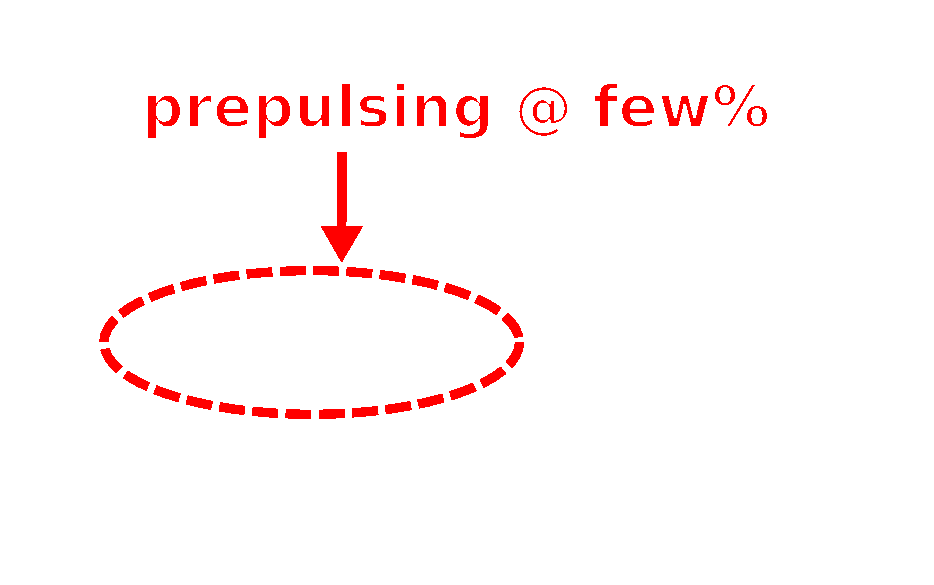
\includegraphics[width=\linewidth]{analyzed_rtq_atm_muon_run005000_test_hitTimePositions_all-prepulse.pdf}};
			\end{tikzpicture}
			\begin{itemize}
				\item<3-> {\fontsize{10pt}{10pt}\selectfont{Prepulsing is few
					\si{\percent} effect.}}
				\item<4-> {\fontsize{10pt}{10pt}\selectfont{fitters must to be
					robust against these statistical outliers}}
			\end{itemize}
		\end{block}
	\end{columns}
\end{frame}

\begin{frame}{Problems are...}
	\begin{itemize}
		\item<1-> Light is produced isotropically
		\item<2-> At high energies
		\begin{itemize}
			\item<2-> complicated kinematics
			\item<2-> multiple final-state particles
		\end{itemize}
	\item<3-> {\color{blue}Let's change perspective and think more simple}
	\item<4-> {\color{blue}There are two pieces of information arriving at PMTs}
		\begin{itemize}
			\item<5-> {\color{blue}Time}
			\item<5-> {\color{blue}Charge}
		\end{itemize}
	\end{itemize}
\end{frame}

\subsection{Idea}
\begin{frame}{Fit direction with charge and time}
	\centering
	\begin{columns}[T]
		\column{0.5\linewidth}
		\begin{block}{}
			\begin{tikzpicture}
				\node (img1)
				{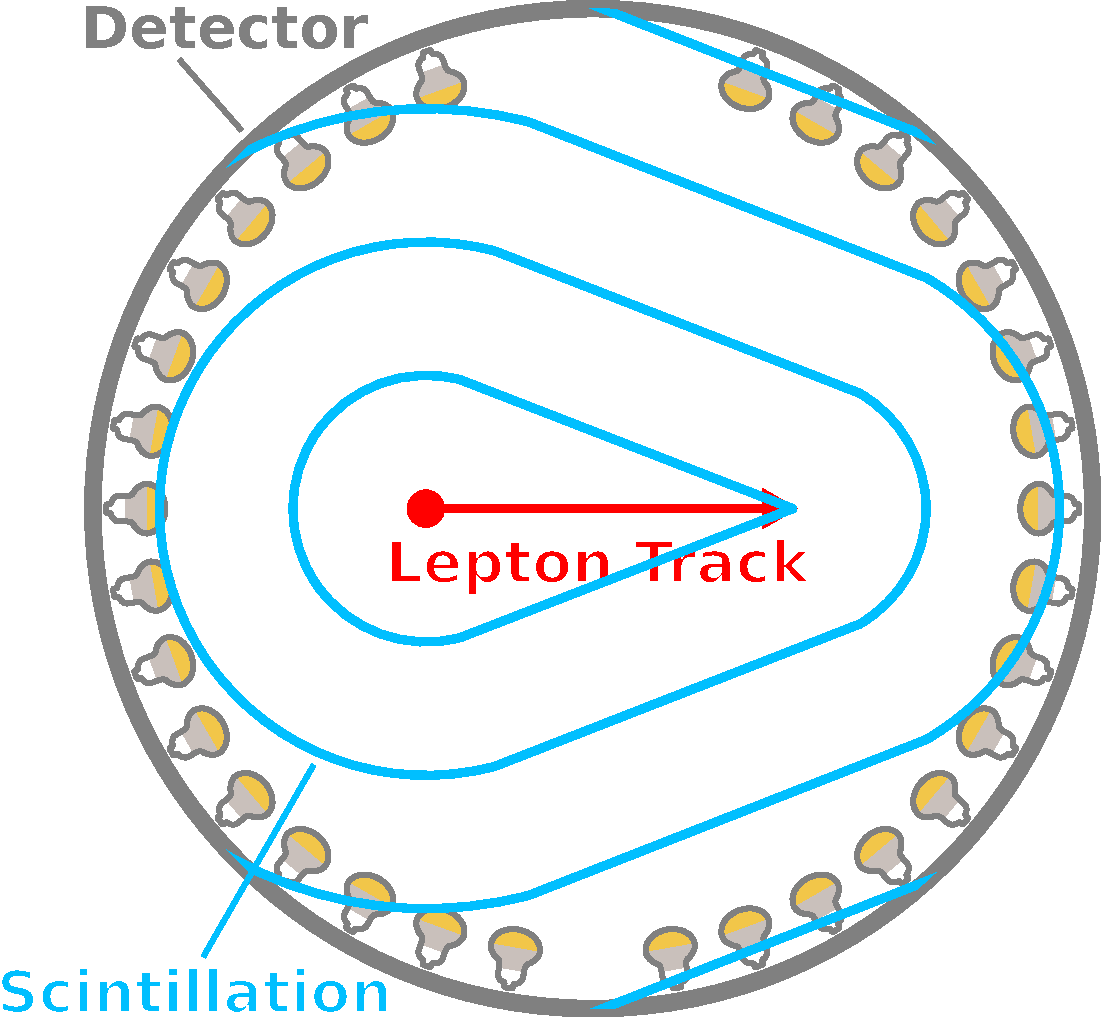
\includegraphics[width=\linewidth]{center_of_charge_and_time.pdf}};
				\pause
				\node (img2) at (img1)
				{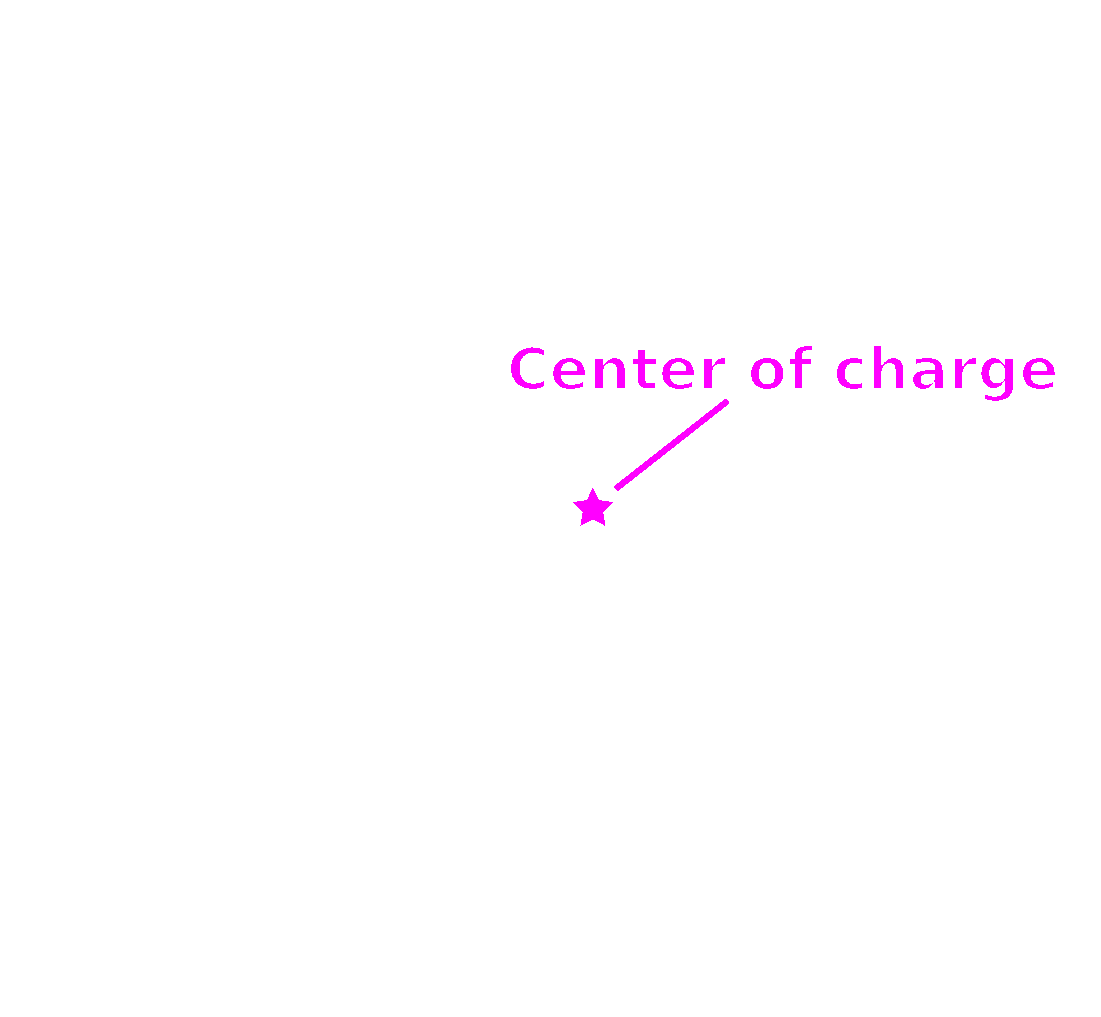
\includegraphics[width=\linewidth]{center_of_charge_and_time-center_of_charge.pdf}};
				\pause
				\node (img3) at (img1)
				{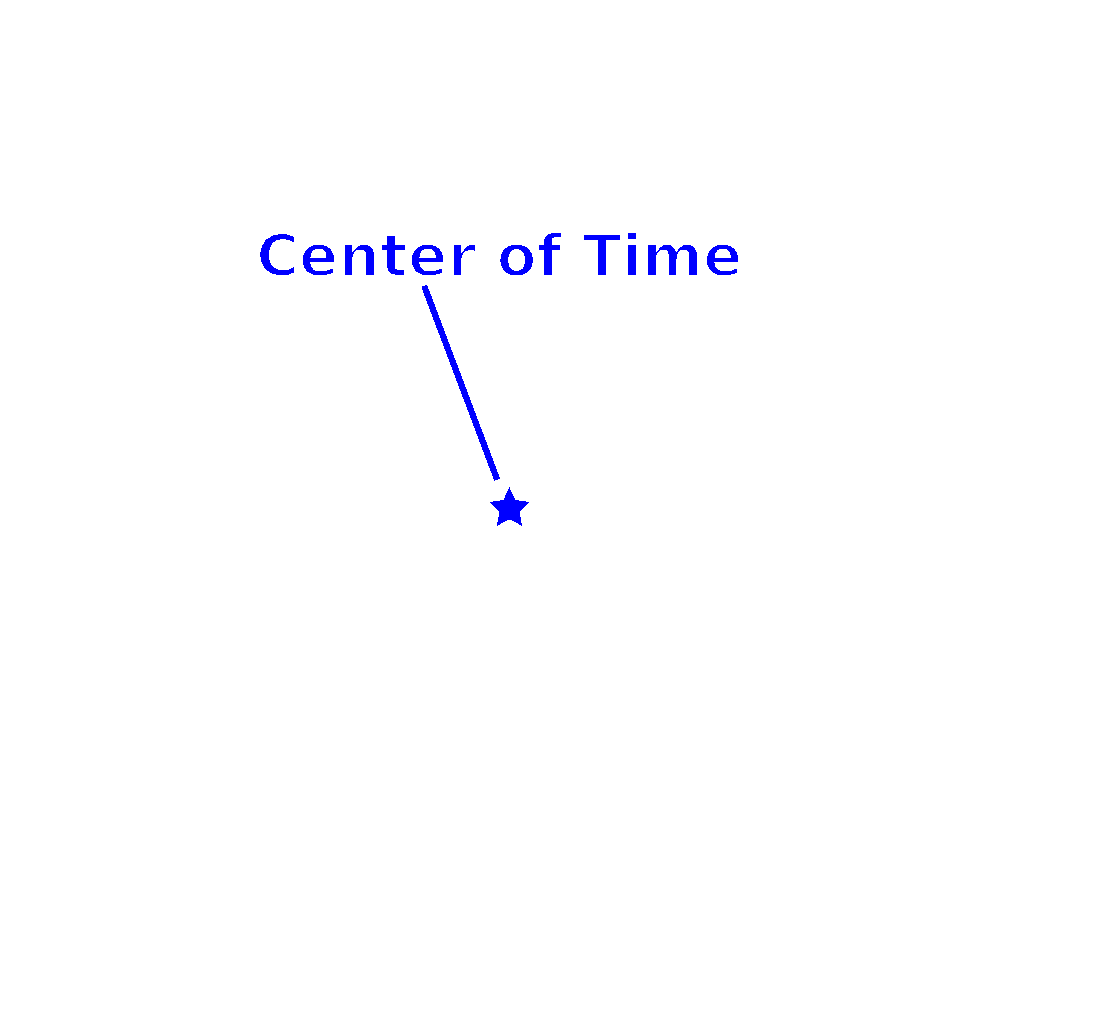
\includegraphics[width=\linewidth]{center_of_charge_and_time-center_of_time.pdf}};
			\end{tikzpicture}
		\end{block}
		\column{0.5\linewidth}
		\begin{itemize}
			\item<2-> Use {\color{magenta}center of charge} to fit middle of
				track
			\item<3-> Use {\color{blue}center of time} to fit near one end of
				track
			\item<4-> And just connect dots to find direction!
		\end{itemize}
	\end{columns}
\end{frame}

\begin{frame}{Question:}
	\begin{itemize}
		\item<2-> {
				But, what do we use for the \underline{weights} in the
				\textbf{weighted~mean}:
				\begin{equation*}
					\frac{\sum_{i}w_{i}x_{i}}{\sum_{i}w_{i}}\,,
				\end{equation*}
				when calculating center of {\color{magenta}\underline{charge}} and
				{\color{blue}\underline{time}}?
			}
		\item<3-> Let's review some basic physics
	\end{itemize}
\end{frame}

\begin{frame}{What weight is used for \emph{center of gravity}?}
	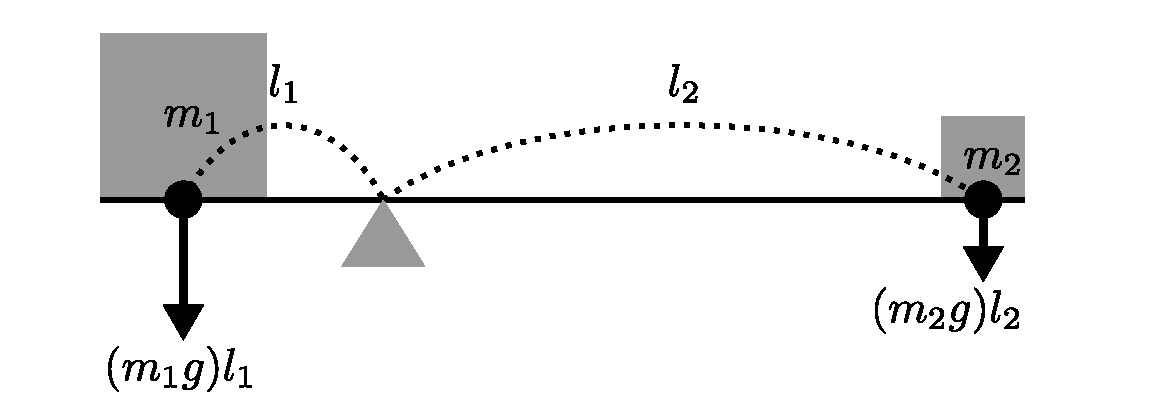
\includegraphics[width=\linewidth]{simple_example_of_center_of_gravity.pdf}
	\begin{itemize}
		\item[]<2-> To find center of gravity:
		\item[]<2-> net torque $= -(m_1 g) l_1 + (m_2 g) l_2 = 0$
		\item[]<3-> $\implies -m_1 l_1 + m_2 l_2 = 0$
		\item[]<4-> $\therefore$ weight is mass: $w_{i} = m_{i}$
	\end{itemize}
\end{frame}

\begin{frame}{What weight is used for \emph{\color{magenta}center of charge}?}
	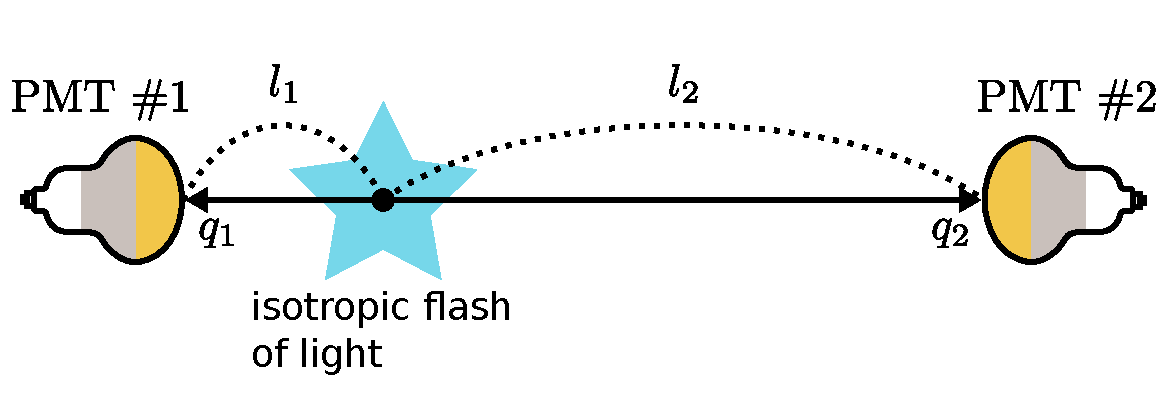
\includegraphics[width=\linewidth]{simple_example_of_center_of_charge.pdf}
	\begin{itemize}
		\item[]<2-> $q_1 \propto \frac{1}{l_1^2}, \quad q_2 \propto
			\frac{1}{l_2^2}$
		\item[]<3-> $\implies \sqrt{q_1} \propto \frac{1}{l_1}, \quad \sqrt{q_2}
			\propto \frac{1}{l_2}$
		\item[]<4-> $\implies -\sqrt{q_1}{l_1} + \sqrt{q_2}{l_2} = 0$
		\item[]<5-> $\therefore$ weight is square root of charge: $w_{i} =
			\sqrt{q_{i}}$
	\end{itemize}
\end{frame}

\begin{frame}{What weight is used for \emph{\color{blue}center of time}?}
	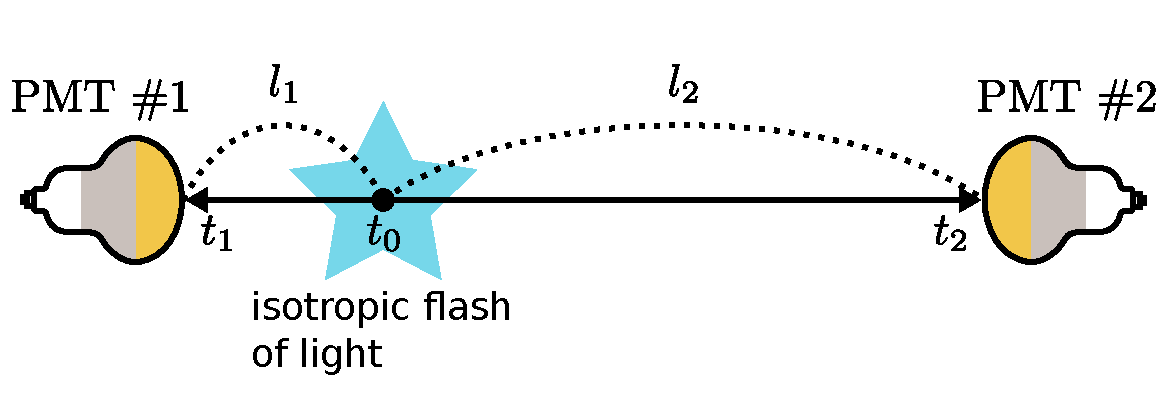
\includegraphics[width=\linewidth]{simple_example_of_center_of_time.pdf}
	\begin{itemize}
		\item[]<2-> Let $\Delta t_i \equiv t_i - t_0$
		\item[]<2-> $\implies \Delta t_1 = \frac{l_1}{c},\quad\Delta t_2 =
			\frac{l_2}{c}$
		\item[]<3-> $\implies -(\frac{1}{\Delta t_1})\frac{l_1}{c} +
			(\frac{1}{\Delta t_2})\frac{l_2}{c} = 0$
		\item[]<4-> $\implies -(\frac{1}{\Delta t_1})l_1 +
			(\frac{1}{\Delta t_2})l_2 = 0$
		\item[]<5-> $\therefore$ weight is inverse of time: $w_{i} =
			\frac{1}{\Delta t_{i}}$
	\end{itemize}
\end{frame}

\begin{frame}{Conclusion}
	\begin{itemize}
		\item<1-> Use \textbf{mass} as weight for \emph{center of gravity}.
		\item<2-> Use \textbf{$\sqrt{\text{charge}}$} as weight for
			\emph{\color{magenta}center of charge}.
		\item<3-> Use \textbf{$\left(\dfrac{1}{\text{time}}\right)$} as weight
			for \emph{\color{blue}center of time}.
	\end{itemize}
\end{frame}

\subsection{Validation}
\begin{frame}{Test algorithm against $\mu$ (Data)}
	\begin{columns}[T]
		\column{0.5\linewidth}
		\begin{block}{\centering{Cosmic ray $\mu$}}
			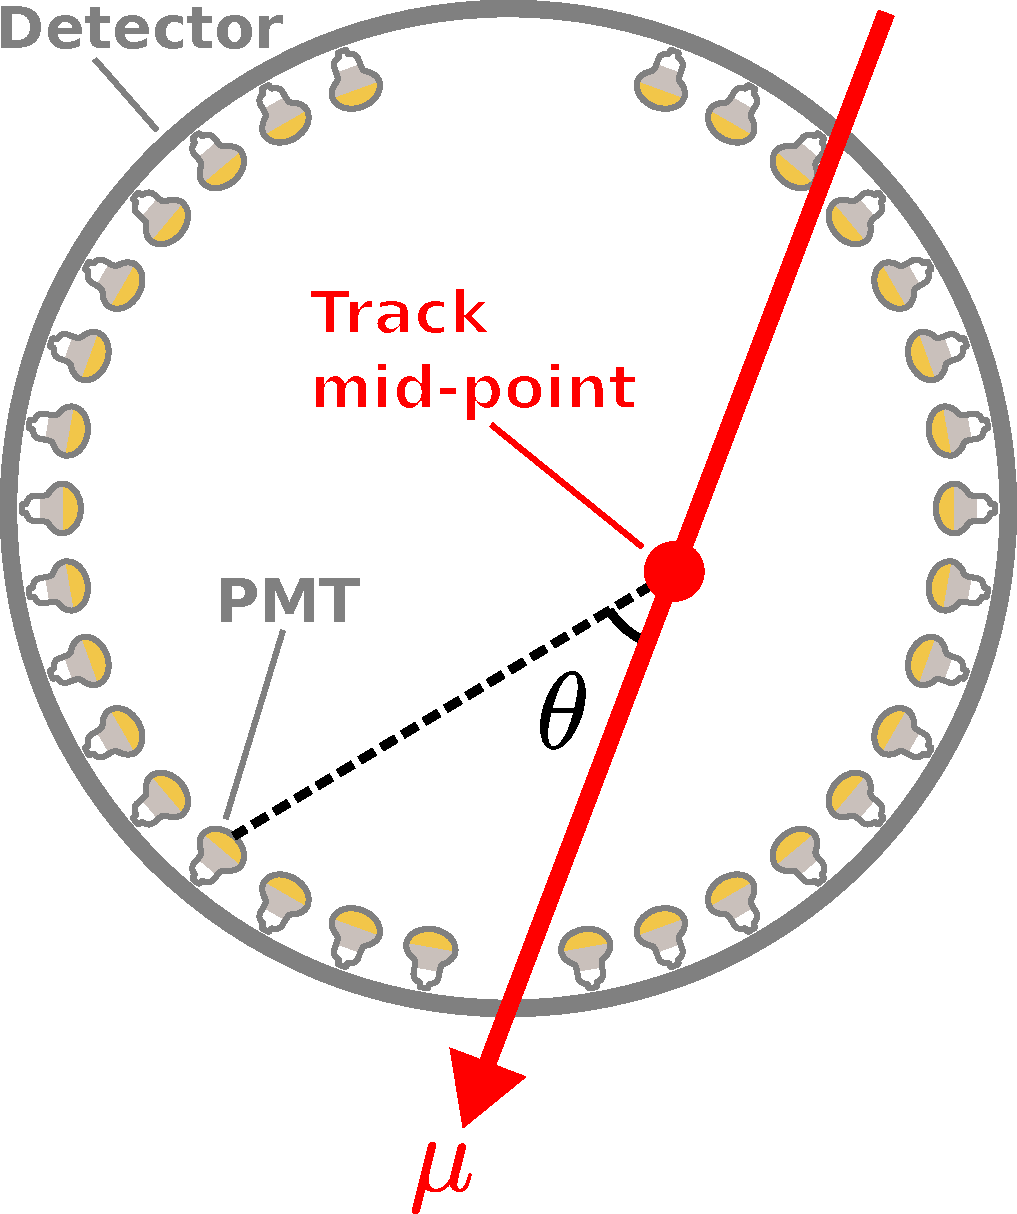
\includegraphics[width=\linewidth]{through_going_muon.pdf}
		\end{block}
		\column{0.5\linewidth}
		\begin{block}{\centering{Deviation from $\mu$-fitter}}
			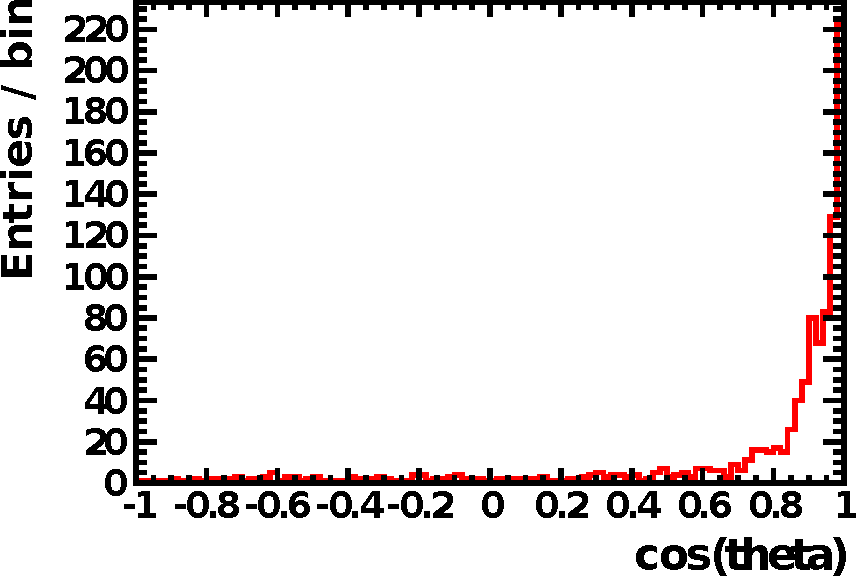
\includegraphics[width=\linewidth]{analyzed_rtq_run005000_agreementWithMuonFitter_t0Peak_prepulseCut1_0_05maxQThres_1000evts.pdf}
		\end{block}
	\end{columns}
\end{frame}

\begin{frame}{Test algorithm against $\Pnu$ (MC)}
	\begin{columns}[T]
		\column{0.5\linewidth}
		%\begin{block}{CC $\Pnue$ interaction on \ce{^1H}}
		\begin{block}{\centering{\ce{{\Pnue} + ^{1}H ->[CC] {\Pelectron} +}}}
			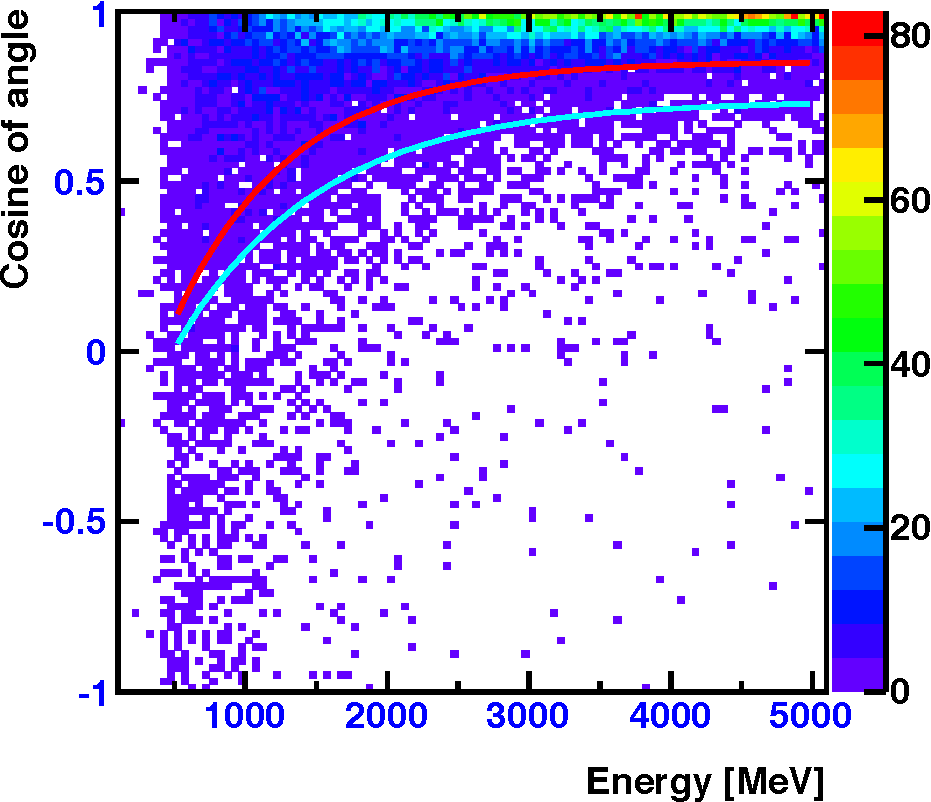
\includegraphics[width=\linewidth]{analyzed_mtq_flatSpectrum_nue_H1_outerBufferFillAll_reconDirAgreementWithMtqTruthVectorVSEnergy_onlyCC_maxR600cm.pdf}
		\end{block}
		\column{0.5\linewidth}
		\begin{block}{\centering{\ce{{\Pnue} + ^{12}C ->[CC] {\Pelectron} +}}}
			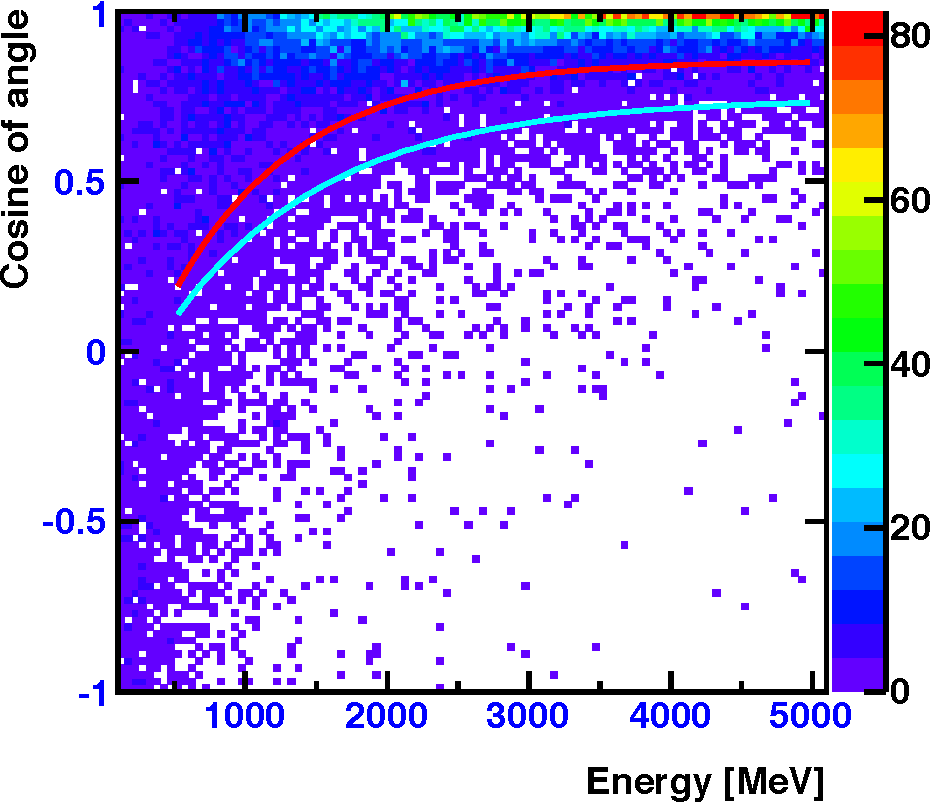
\includegraphics[width=\linewidth]{analyzed_mtq_flatSpectrum_nue_C12_outerBufferFillAll_reconDirAgreementWithMtqTruthVectorVSEnergy_onlyCC_maxR600cm.pdf}
		\end{block}
	\end{columns}
	\begin{itemize}
		\item Black line: \SI{1}{\sigma} of reconstructed angle from \Pnu
			direction
		\item Red line: \SI{1}{\sigma} of lepton angle from \Pnu direction
	\end{itemize}
\end{frame}

\begin{frame}{Test algorithm against T2K events (Data)}
	\begin{columns}[T]
		\column{0.5\linewidth}
		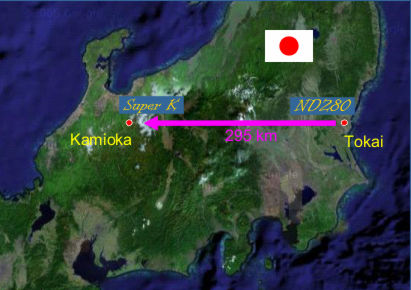
\includegraphics[width=\linewidth]{t2k.jpeg}
		\column{0.5\linewidth}
		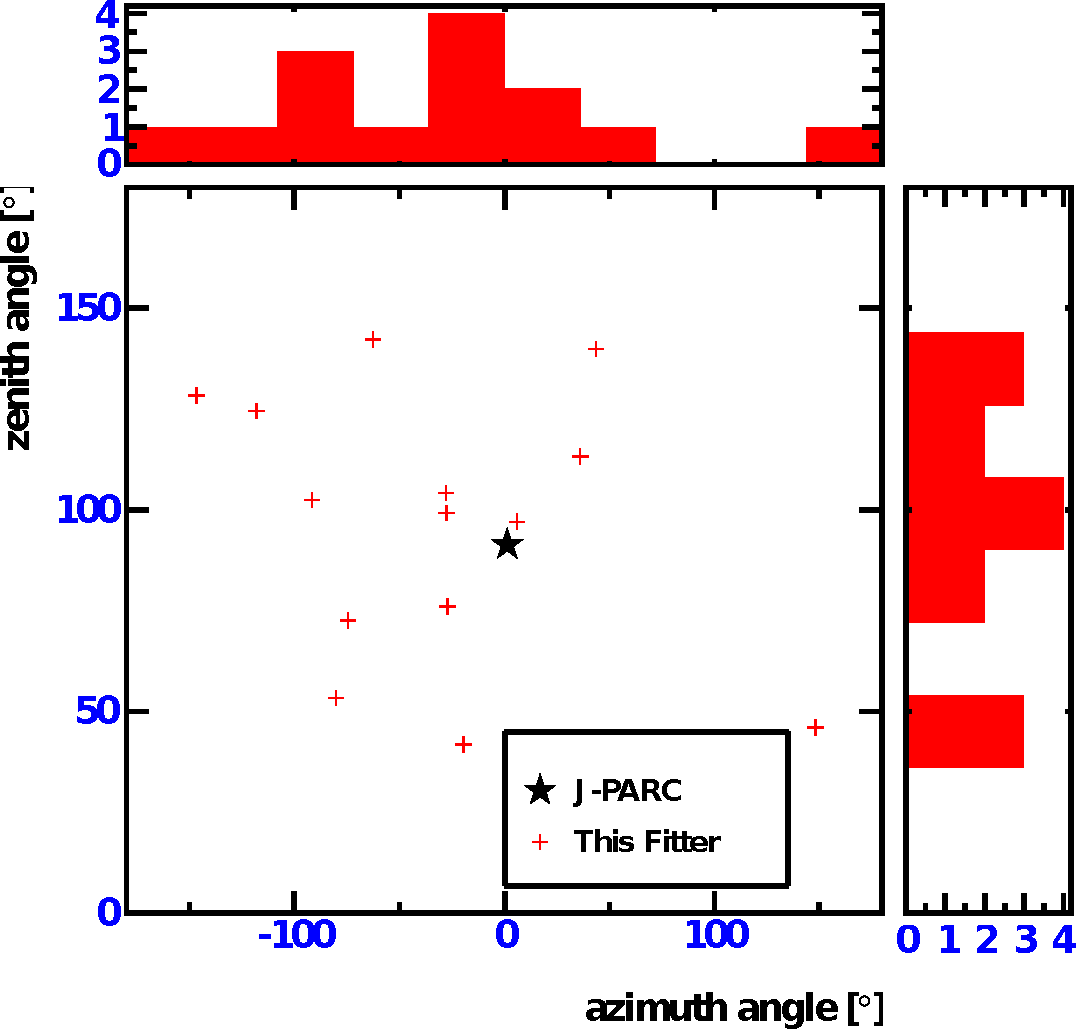
\includegraphics[width=\linewidth]{analyzed_rtq_t2k_nu_noNegativeCharge_prepulseCut_t2kReconDir.pdf}
	\end{columns}
\end{frame}

\begin{frame}{Test algorithm against T2K events (Data)}
	\begin{columns}[T]
		\column{0.5\linewidth}
		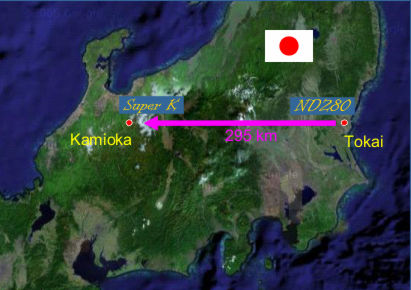
\includegraphics[width=\linewidth]{t2k.jpeg}
		\column{0.5\linewidth}
		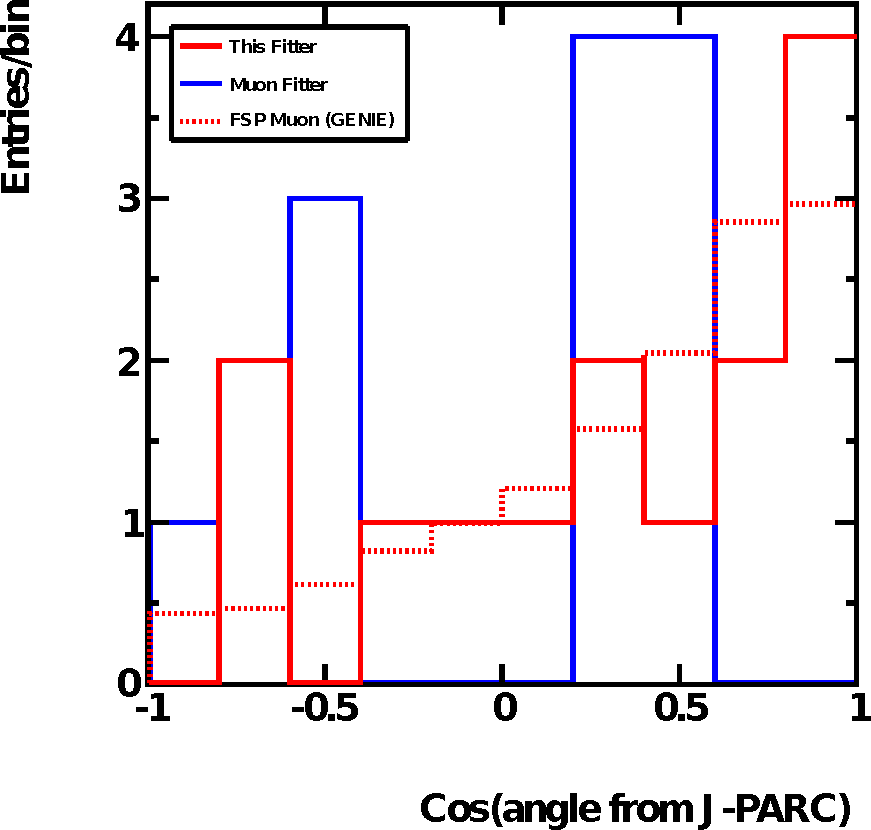
\includegraphics[width=\linewidth]{analyzed_rtq_t2k_nu_t2kReconDir_hist.pdf}
	\end{columns}
\end{frame}

\section{Track reconstruction and particle discrimination}
\begin{frame}
	\centering
	Track Reconstruction and Particle ID
\end{frame}

\subsection{Algorithm}
\begin{frame}{Hellgartner's algorithm}
	\begin{equation*}
		h(\vec{x}, t) = \sum_{i=1}^{N_{\text{PMT}}}
		\Theta(q_i - q_{\text{threshold}})
		\sum_{j=1}^{N_{\gamma}} f(t_{ij} - t_{i}^{\text{TOF}}, t) \,
	\end{equation*}
	{\footnotesize
		where
		$N_{\text{PMT}}$: number of PMTs\\
		$N_{\gamma}$: number of photon hits to count per PMT\\
		$q_i$: charge on $i$-th PMT, $q_{\text{threshold}}$: minimum charge for
		analysis\\
		$t_{ij}$: $j$-th hit time on $i$-th PMT\\
		$t_i^{\text{TOF}}$: expected time-of-flight between $i$-th PMT and
		$\vec{x}$
	}
	\begin{equation*}
		f(\Delta t, t) \propto (t - \Delta t) \exp{\bigg[-\frac{(\Delta t -
		t)^2}{2 \sigma_{\text{tts}}}\bigg]}
	\end{equation*}
	\begin{equation*}
		\text{{\normalsize\textbf{\underline{Figure of merit}}} {\footnotesize
		for each test point in space}} = \int_{-\infty}^{\infty} |h(\vec{x}, t)|^2 \,\mathrm{d}t
	\end{equation*}
\end{frame}

\subsection{Validation}
\begin{frame}{\normalsize Test Hellgartner on double
	$\SI{1}{\giga\electronvolt}$ muons (MC)}
	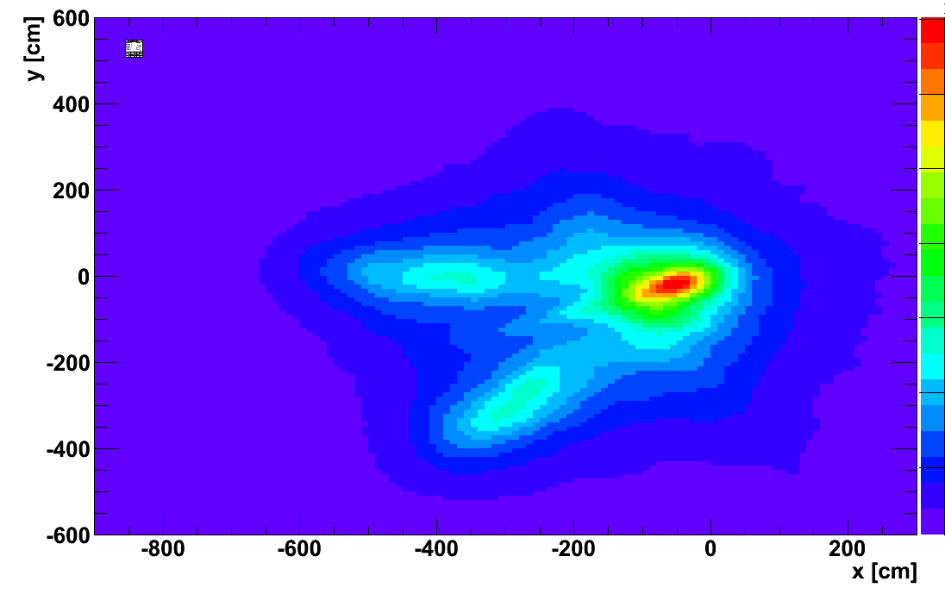
\includegraphics[width=\linewidth]{hellgartner_double_muon.pdf}

	{\footnotesize Dominikus Hellgartner}
\end{frame}

\begin{frame}{Test Hellgartner on
	$\SI{2}{\giga\electronvolt}$ \Pnue (MC)}
	\centering
	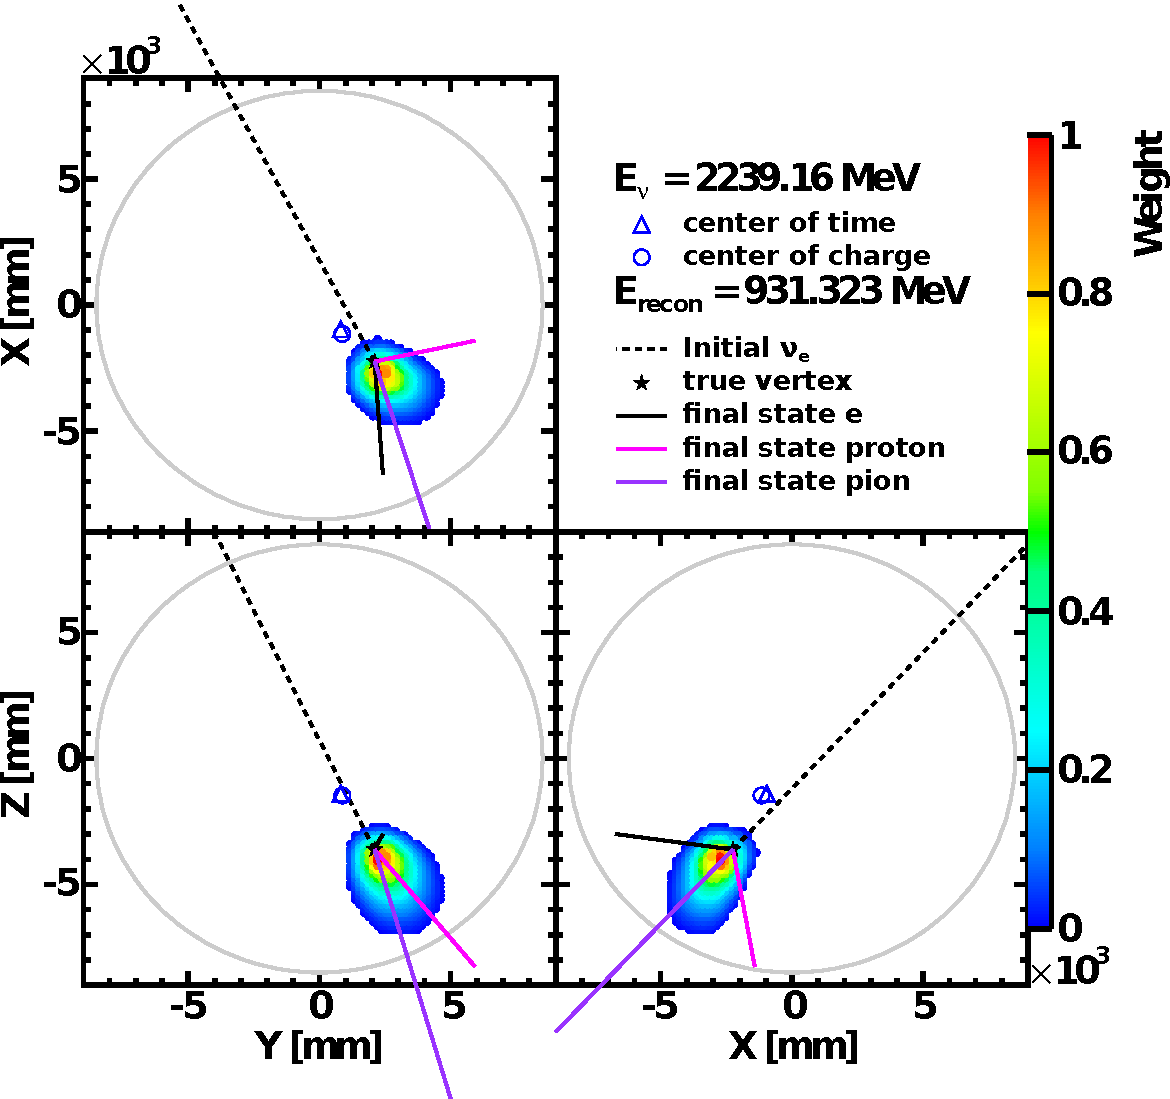
\includegraphics[width=0.8\linewidth]{hellgartner_reconstruction_2gev_nue_klg4sim.pdf}
\end{frame}

\begin{frame}{Test Hellgartner on T2K events (Data)}
	\centering
	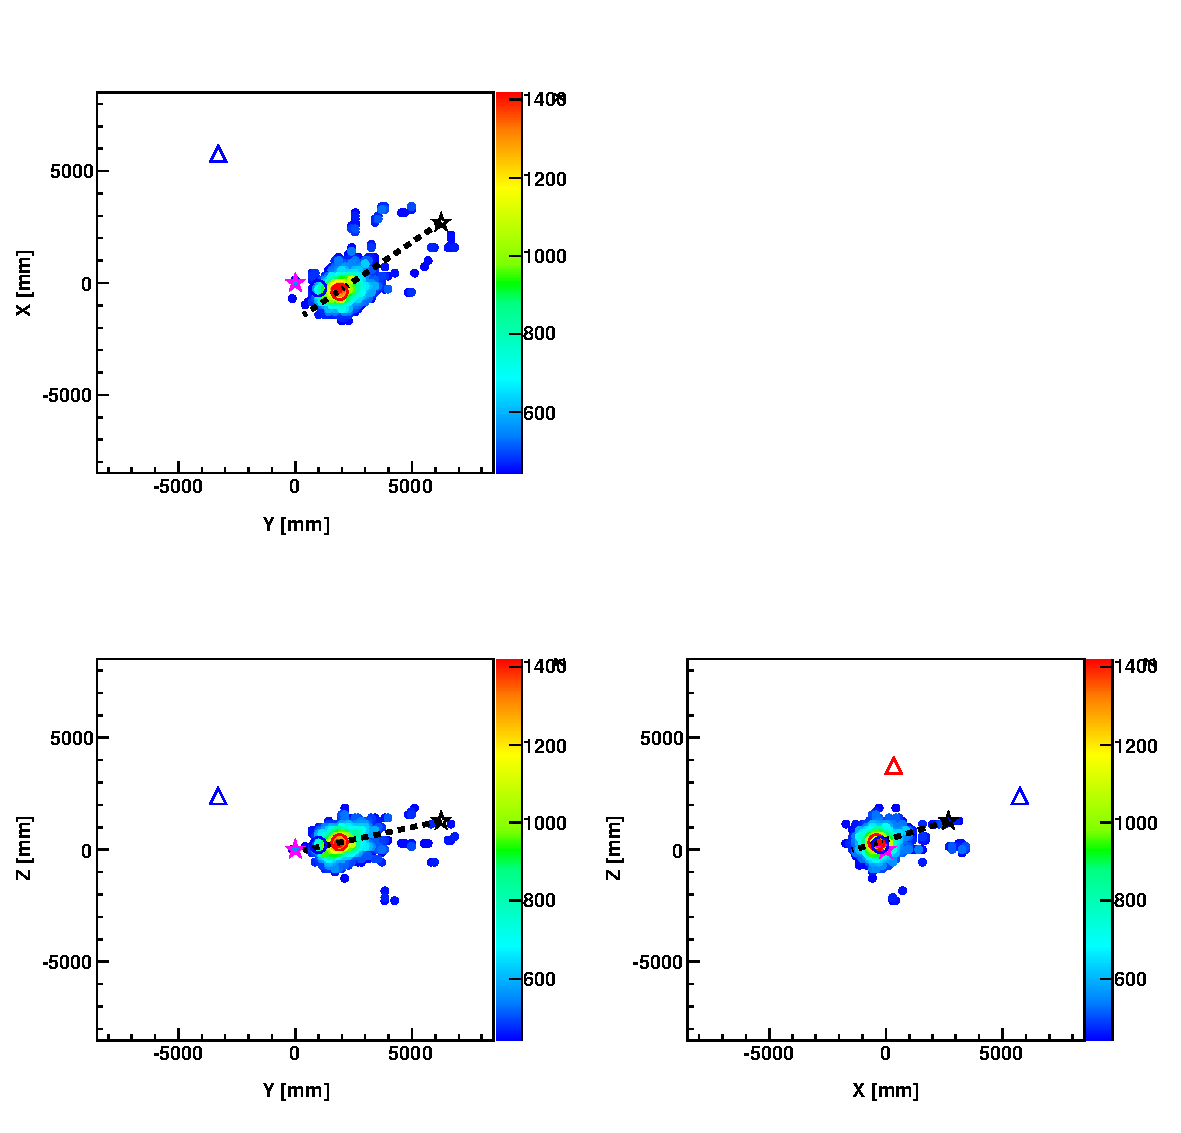
\includegraphics[width=0.8\linewidth]{fom_map__run11331_evt29962767.pdf}
\end{frame}

\begin{frame}{Lepton discrimination algorithm}
	Explanation is here.
\end{frame}

\begin{frame}{Test lepton discrimination (MC)}
	\centering
	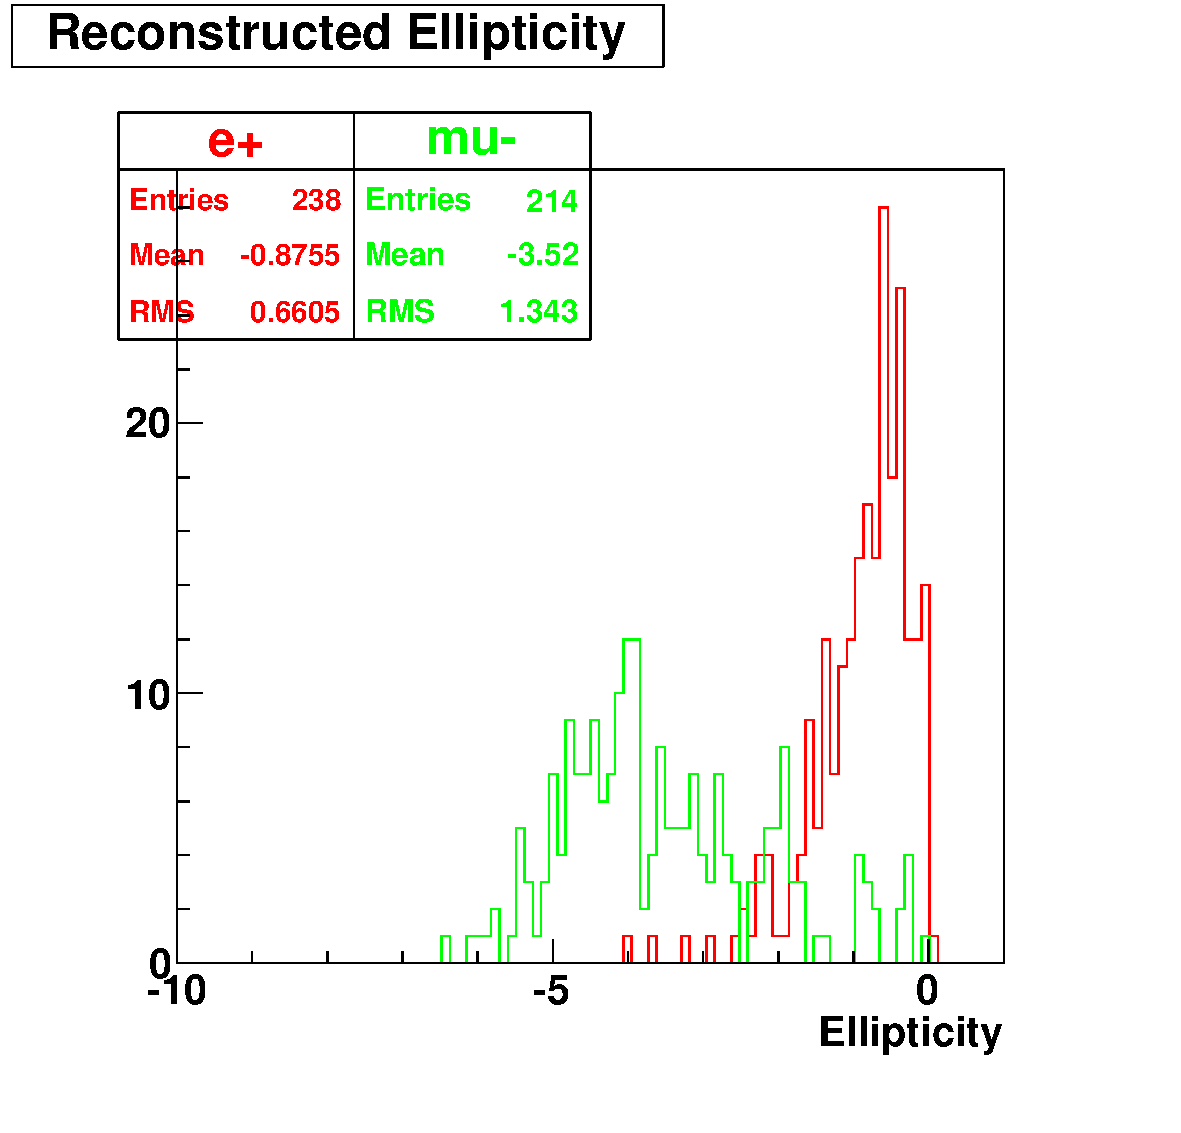
\includegraphics[width=0.8\linewidth]{emu_mtq_recon_ellipticity-3Mcut.pdf}
\end{frame}

\end{document} 
